\chapter{Trabalhos Relacionados}\label{ch:Relacionados}


O Abuso Sexual Infantil (ASI) maninesta-se como um problema global. Diante disso, profissionais da saúde e pesquisadores passaram a se dedicar a compreender as raízes  deste mal que assola milhares de crianças todos os anos \cite{deslandes1994atenccao, dahlberg2006violencia, da2017violencia}. A área de criminologia em específico, desenvolveu uma série de teorias acerca das causas para os atos infracionais. Dentre elas, destaca-se a Teoria da Atividade Rotineira, ilustrada na \autoref{fig:Crime}.
%Inúmeros métodos surgiram para compreender as raízes do problema, dentre eles, cita-se a Análise de Causa Raiz (ACR). Tal método visa descobrir a causa de um problema para identificar soluções adequadas \cite{rooney2004root}.

\begin{wrapfigure}{r}{7.1cm}
  \caption{\label{fig:Crime}Triângulo do Crime}
      \begin{center}
        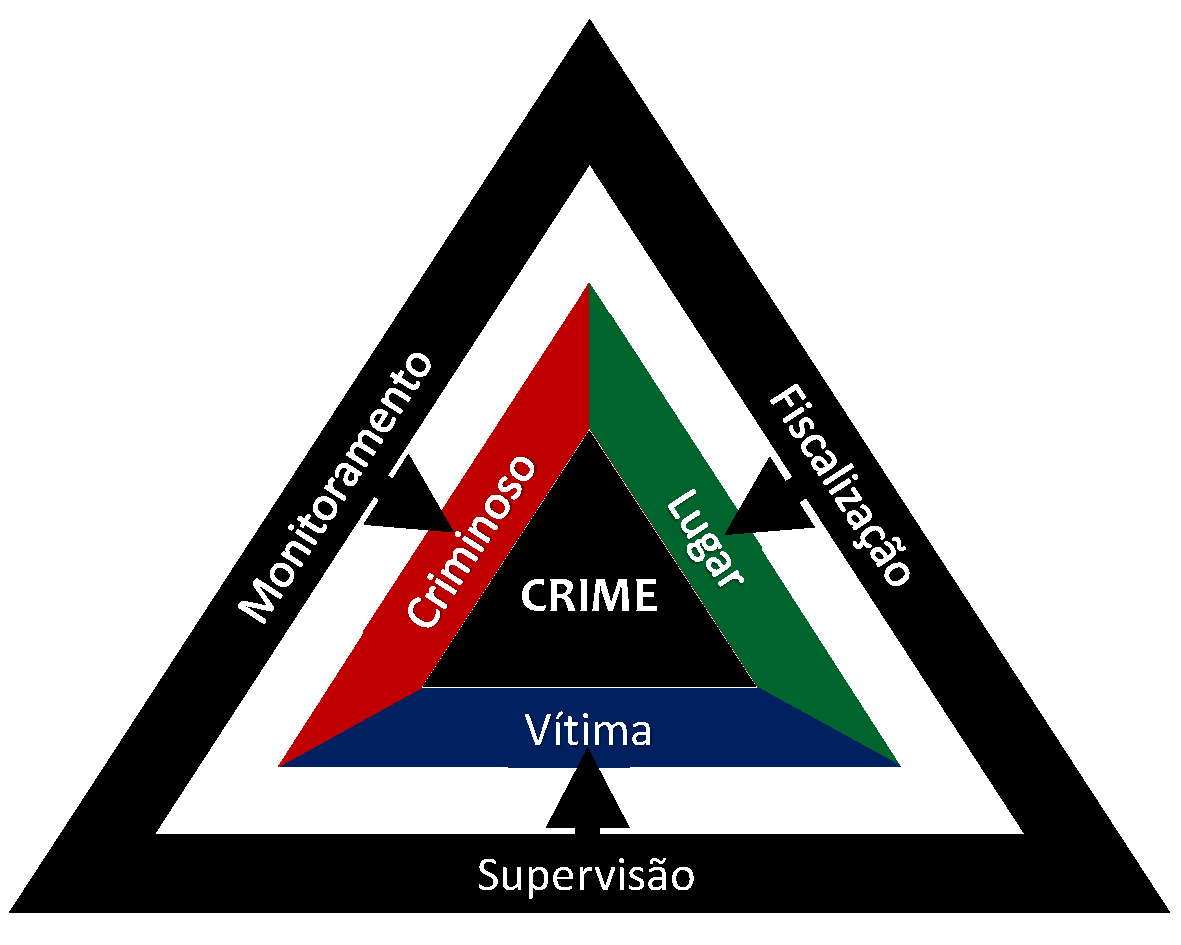
\includegraphics[width=\linewidth]{./Figuras/TrianguloCrime.pdf}
      \end{center}
      \legend{Fonte: os autores}
\end{wrapfigure}

O infográfico da \autoref{fig:Crime} apresenta os três elementos básicos da Teoria da Atividade Rotineira, também conhecida como Triângulo do Crime. Em resumo, três elementos são considerados essenciais para a ocorrência de um crime. Para que um crime aconteça deve-se haver um criminoso motivado sem supervisão, um lugar sem fiscalização e um vítima desprotegida ou vulnerável. Tomar atitudes preventivas sob qualquer um destes elementos, dificulta a ocorrência do crime. Todavia, destaca-se que estes elementos não possuem pesos iguais, mas sim, se interbalanceiam entre si (e.g. em certas condições, um lugar bem fiscalizado poderia não ser um empecilho para um criminoso muito motivado).



%criminoso = supervisão
%lugar = fiscalização
%Vítima = proteção

O Triângulo do Crime apresenta as três partes fundamentais para a ocorrência de um crime. As estratégias de combate ao abuso sexual infantil se objetivam a agir sob estas partes fundamentais. Algumas estratégias são focadas no monitoramente de criminosos\footnote{\label{note:nota1}Círculos de Suporte e Responsabilidade (Em inglês: Circles of Accountability and Support - CoSA) são grupos de voluntários com supervisão profissional para apoiar os agressores sexuais à medida que se reintegram à sociedade após serem libertados do encarceramento.}, outras no fortalecimento da fiscalização de espaços públicos ou privados\footnote{Lei nº 12.038, de 1º de outubro de 2009 dificulta a exploração sexual de crianças e adolescente impossibilitando a hospedagem deles por terceiros que não apresentem autorizações legais.}, e outras na capacitação preventiva de potenciais vítimas, tornando-as menos vulneráveis\footnote{O programa educacional Talking about Touching é um programa focado no ensino de habilidades básicas para crianças com finalidade de ajudá-las a se protegerem de situações abusivas.}. Cada estratégia pode ser dividida com base em seus níveis de prevenção. Os níveis de prevenção são apresentados em maiores detalhes na \autoref{fig:prevencao}.

\begin{figure}[htb]
	\caption{\label{fig:prevencao}Níveis de Prevenção}
  \begin{center}
    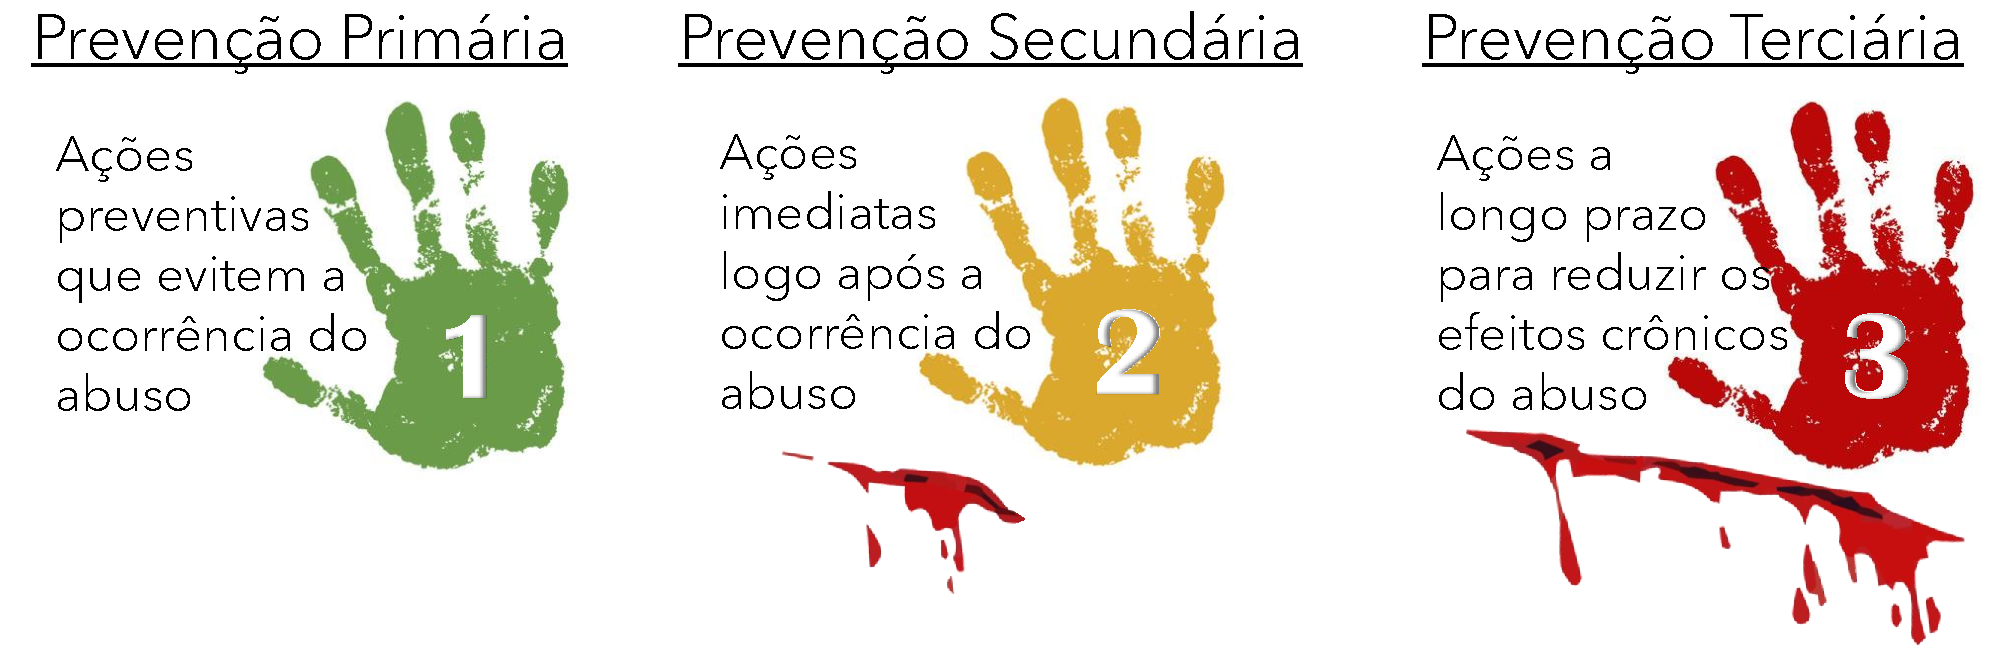
\includegraphics[width=\linewidth]{./Figuras/Prevencao.pdf}
	\end{center}
	\legend{Fonte: os autores}
\end{figure}

A \autoref{fig:prevencao} apresentada os três níveis de prevenção mais comumentes relatados na literatura pesquisada. São eles: prevenção primária, prevenção secudária e prevenção terciária \cite{dahlberg2006violencia, santos2011guia, maria2012abusos}. No caso do abuso sexual infantil, a prevenção primária engloba iniciativas que antecipam a incidência do abuso sexual contra crianças e adolescentes  \cite{marcelino2017vamos}. A prevenção secundária enfatiza uma resposta imediata após a ocorrência da violência sexual. Já a prevenção terciária corresponde, de modo geral, a ações de longo prazo para o tratamento e recuperação das vítimas \cite{people2020expert}. Informa-se que a literatura médica relata também um quarto nível de prevenção. A prevenção quartenária descreve sobre ações preventivas contra eventuais exageros na utilização de métodos preventivos \cite{tesser2017importante}. Embora presente na literatura médica, salienta-se que a atual dissertação engloba apenas os três níveis de prevenção mais relatados pela bibliografia pesquisada acerca do abuso sexual infantil.

Os níveis de prevenção do abuso sexual infantil não se resumem a atuar apenas sob as crianças. Há registros de prevenção terciária relacionados inclusive ao tratamento/acompanhamento de agressores sexuais\footref{note:nota1}. O combate ao abuso sexual infantil assume então inúmeras facetas, cada qual, objetivada a diminuir de alguma forma os fatores de risco que influênciam a ocorrência de violações sexuais.

Os Fatores de Risco são aquelas circunstâncias que aumentam a probabilidade da ocorrência de um episódio de violência. Deste modo, o abuso infantil apresenta mais chances de ocorrer quando os fatores de risco se acumulam. Os Fatores de Risco interagem entre si, no que é chamado de risco em cascata, no qual um risco inicial pode acompanhar ou desencadear outros riscos, terminando por resultar em um acúmulo sucessivo de fatores de risco \cite{Recommendations2019Taylor}. A \autoref{fig:Riscos} apresenta a disposição dos fatores de riscos mais apontados pela literatura na área por meio de um Modelo Ecológico. 

%O modelo socio-ecológico é uma estrutura de saúde pública desenvolvida pelos Centros de Controle e Prevenção de Doenças (em inglês: Centers for Disease Control and Prevention - CDC) \cite{centers2019social}. O modelo socio-ecológico data desde a década de 1970, sendo  aplicado aos casos de abuso infantil \cite{dahlberg2006violencia}. O modelo explora a relação entre os fatores individuais e contextuais e considera a violência como produto dos múltiplos níveis de influência sobre o comportamento


%https://www.scielo.br/pdf/csc/v11s0/a07v11s0.pdf \cite{dahlberg2006violencia}

%https://www.unicef.org/media/66741/file/Promising-programme-responses.pdf4 \cite{topromising}

%https://www.k12.wa.us/sites/default/files/public/hivsexualhealth/pubdocs/Erin%27s%20Law%20Report.pdf [fez que nem eu] \cite{Recommendations2019Taylor}

%https://www.doh.wa.gov/Portals/1/Documents/Pubs/140-165-SexualViolencePreventionPlan.pdf [fez que nem eu] \cite{sexual2017department}

%https://www.cdc.gov/violenceprevention/pdf/svprevention-a.pdf \cite{centers2004sexual}

\begin{figure}[htb]

	\caption{\label{fig:Riscos}Modelo Ecológico}
  \begin{center}
    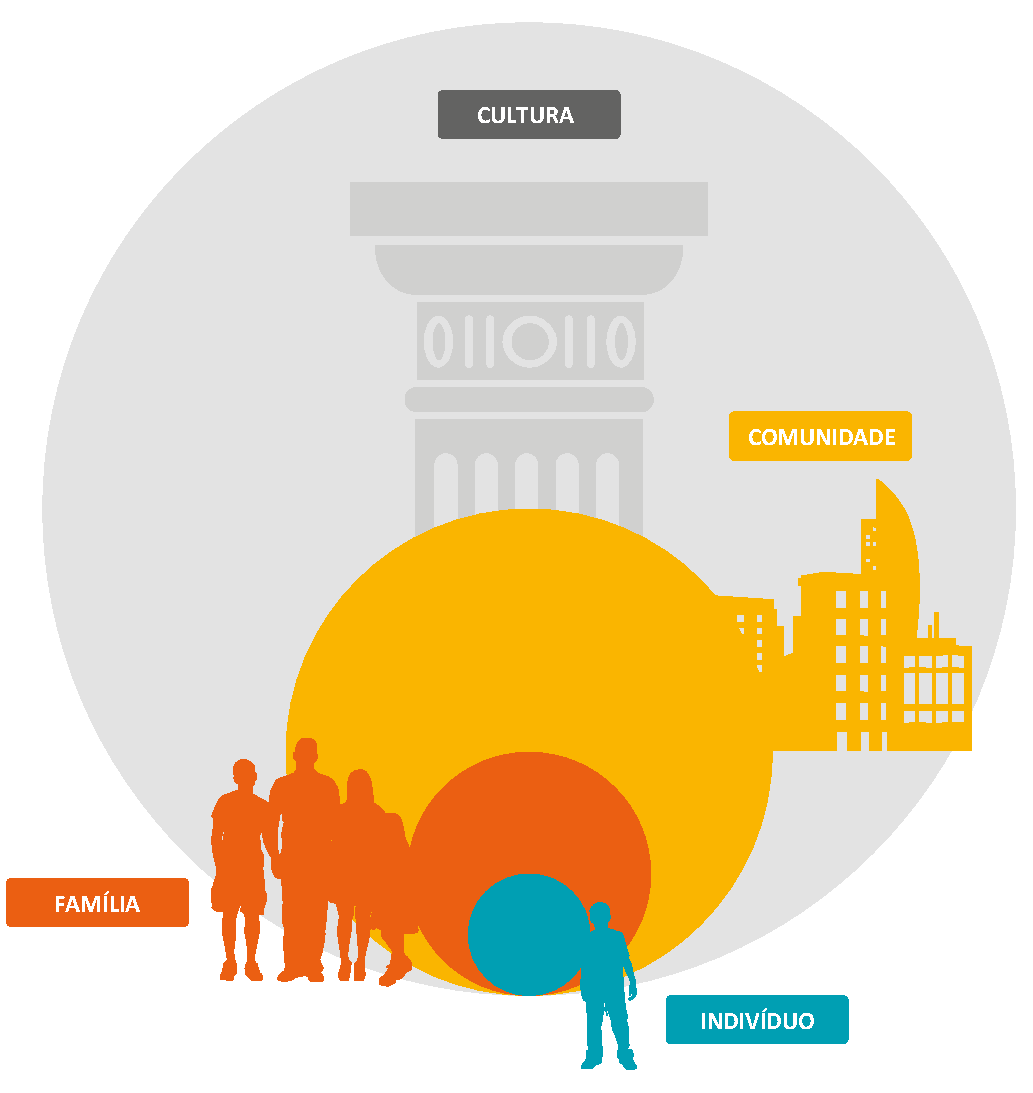
\includegraphics[width=0.75\linewidth]{./Figuras/FatoresRisco.pdf}
	\end{center}
  \legend{Fonte: adaptado de \cite{blasco2018abuso}}

\end{figure}
%https://www.savethechildren.es/sites/default/files/imce/docs/mas_me_duele_a_mi.pdf
%[ainda sita-se a falta de sensibilização da sociedade, lideres politicos, etc tec.... pag 39]

O Modelo Ecológico da \autoref{fig:Riscos} ilustra os quatros fatores de risco mais presentes na bibliografia pesquisa. Salienta-se que os fatores de risco podem váriar em quantidade e em nomenclatura, dependendo da fonte literária \cite{centers2004sexual, sexual2017department, blasco2018abuso, topromising}. Todavia, a ideia base do Modelo Ecológico tendem a permanecer inalterada. O modelo em si, explora a relação entre os fatores individuais e contextuais que acabam por implicar em um cenário de violência \cite{dahlberg2006violencia}. Os fatores de risco do abuso sexual infantil mais influentes são:

\begin{itemize}
  \item \textbf{Indivíduo:} \hfill Aspectos individuais que fomentem a ocorrência do abuso sexual. %Válido tanto para as vítimas quanto para os agressores. 
  \item \textbf{Família:} \hfill Questões familiares que viabilizam as condições para a violência.  %circunstâncias
  \item \textbf{Comunidade:} Condições econômicas e governamentais que propiciem o abuso.
  \item \textbf{Cultura:} \hfill Crenças sociais que estimulem atividades sexuais com menores. 
\end{itemize}


Os fatores de risco podem interatuar entre si de modo a maximizar as chances de um evento abusivo. O baixo nível educacional de um \textbf{Indivíduo} é um dos elementos a ser citado neste aspecto \cite{dahlberg2006violencia}. A negligência da \textbf{Família} nos cuidados infantis é outro aspecto a ser citado \cite{blasco2018abuso}. Cita-se também, a premisividade do casamento infantil de algumas \textbf{Culturas} \cite{bandiera2017women}. Assim, como a baixa condição sócio-econômica de uma \textbf{Comunidade}. A exemplo, soros positivos de comunidades africanas veem o relaciomento sexual com crianças como um ato de limpeza e cura da síndrome de imunodeficiência adquirida \cite{aded2006abuso}.

%Na Africa, ``as crianças correm grande risco de contaminação pelo vírus HIV''.. existe a crença que os portadores serão limpados da doença. \cite{aded2006abuso} [possivelmente falar sobre isso na hora de falar do treinamento para os pais]

%``We evaluate a \textbf{multifaceted policy intervention} attempting to jumpstart adolescent women’s empowerment in Uganda'' ... ``Strikingly, the share of girls reporting sex against their will drops by close to a third and aspired ages at which to marry and start childbearing move forward.'' \cite{bandiera2017women} [BRAC-ELA as a tool to aid womens’ empowerment]

Agir sobre os fatores de risco (\autoref{fig:Riscos}), implica em agir de forma mais efetiva no combate a violência sexual infantil. Compreender os níveis de prevenção (\autoref{fig:prevencao}), implica em compreender os momentos de atuar sobre o problema. Entender as raízes da violência (\autoref{fig:Crime}), implica em entender seus elementos operantes. Estudar o problema do abuso sexual infantil, é necessário para se ter um panorama geral acerca dos possíveis cenários de atuação e combate. Além disso, um levantamento bibliográfico sobre as estratégias de combate já desenvolvidas se faz indispensável para evitar a perda de tempo e dinheiro no desenvolvimento de uma solução já existente \cite{wazlawick2014metodologia}. 

Este Capítulo elenca as principais soluções utilizadas no combate ao abuso sexual infantil de acordo com a bibliografia pesquisada. O levantamento bibliográfico fundamenta-se nos seguintes mecanismos de busca acadêmica (MBAs): ACM DL, IEEExplore, Science Direct e Web of Science. A escolha por esses MBAs deu-se por abrigarem publicações de qualidade reconhecida pela Coordenação de Aperfeiçoamento de Pessoal de Nível Superior (CAPES) \cite{capes2016}%e por possuírem a maior quantidade de recursos de busca e seleção \cite{buchinger2014mecanismos}
. Também foram pesquisados periódicos, livros, revistas científicas e \textit{sites} de referência na área; além de consultadas as citações referenciadas nesta dissertação. 

Diante do exposto, a presente dissertação divide as Seções deste Capítulo em grupos de soluções utilizadas no combate ao abuso sexual infantil. Cada solução visa mitigar o problema da sua própria maneira. Dentre as soluções apresentadas, informa-se que as soluções baseadas em jogos são abordadas mais profundamente em relação as demais, por se tratarem do cerne da atual pesquisa. Dito isso, a \autoref{sec:regras} descreve normas e legislações sobre os direitos das crianças, a \autoref{sec:canais} apresenta algumas formas de denúncia, a \autoref{sec:propagandas} aponta ações publicitárias, a \autoref{sec:hospital} trata de questões hospitalares, a \autoref{sec:centros} apresenta os centros de atendimento, a \autoref{sec:dp} lista algumas delegacias especializadas, a \autoref{sec:op} elenca operações políciais, a \autoref{sec:infratores} apresenta alguns tratamentos com infratores, a \autoref{sec:programas} menciona alguns programas de capacitação, a \autoref{sec:materiais} relata materias didáticos de ensino e a \autoref{sec:finais} dá as considerações finais do presente Capítulo. 

%\autoref{ssec:pais}
%\autoref{ssec:professores}
%\autoref{ssec:alunos}

%\autoref{ssec:analogico}
%\autoref{ssec:digitais}
%\autoref{ssec:jogos}




%procurando aumentar o conhecimento dos menores na problemática em questão, tornando-as mais resilientes e menos vulneráveis

%, visando mitigar os males iniciais causados por um evento de abuso

%https://repositorio.ufscar.br/bitstream/handle/ufscar/2835/TeseMGSP.pdf?sequence=1&isAllowed=y

%https://www.udesc.br/arquivos/cct/id_cpmenu/1024/disserta_ao_completa_15532596804969_1024.pdf

%https://www.scielo.br/pdf/csc/v11s0/a07v11s0.pdf

%http://portaldoprofessor.mec.gov.br/storage/materiais/0000016936.pdf

%https://www.scielosp.org/article/csc/1999.v4n1/171-181/pt/

%https://repositorio.iscte-iul.pt/bitstream/10071/15660/1/Disserta%c3%a7%c3%a3oDianaMarcelino.pdf

%https://repositorio.iscte-iul.pt/bitstream/10071/12615/3/2016_ECSH_DPSO_Dissertacao_Magda%20Moita.pdf

%https://repositorio.iscte-iul.pt/bitstream/10071/10673/1/2015_ECSH_DPSO_Dissertcao_Nicole%20Christine%20Alves%20Figueiredo.pdf

%https://www.unicef.org/media/66741/file/Promising-programme-responses.pdf4

%http://repositorio.ispa.pt/bitstream/10400.12/1768/1/TES%20MARI1.pdf

%https://www.k12.wa.us/sites/default/files/public/hivsexualhealth/pubdocs/Erin%27s%20Law%20Report.pdf

%https://www.cdc.gov/violenceprevention/pdf/svprevention-a.pdf

%https://www.doh.wa.gov/Portals/1/Documents/Pubs/140-165-SexualViolencePreventionPlan.pdf

%https://bmcpublichealth.biomedcentral.com/articles/10.1186/s12889-017-4502-6

%https://www.gov.scot/publications/expert-group-preventing-sexual-offending-involving-children-young-people-prevention-responses-harmful-sexual-behaviour-children-young-people/pages/11/

%https://www.e-publicacoes.uerj.br/index.php/sustinere/article/view/30004/23155

%https://www.scielosp.org/article/csc/2006.v11suppl0/1163-1178/pt/

%https://endsexualviolencect.org/what-we-do/prevention/primary-prevention/

%e discutir medidas para sua prevenção


%\cite{eck1995examining}

%``Na década de 1980, profissionais da saúde como médicos, pesquisadores e os sistemas de  saúde  pública  passaram  a  se  dedicar  a  compreender  as  raízes  daviolência  e  discutir medidas   para   sua   prevenção.   É   também   nessa   década   que   a   violência   passa   a   ser considerada  um  problema  de  saúde  pública,  devido  ao  aumento  de  mortes  e  traumas  que congestionam os serviços de saúde (DESLANDES, 1994; DAHLBERG e KRUG, 2007).'' %https://www.e-publicacoes.uerj.br/index.php/sustinere/article/view/30004/23155


%\section{Teste $
\includegraphics[width=0.05\linewidth]{./Figuras/Prevencao1.pdf}$$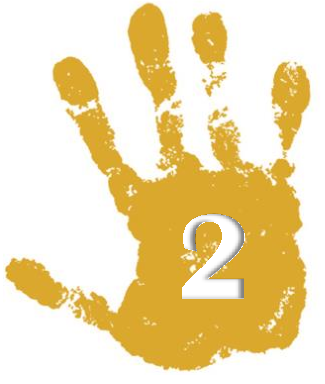
\includegraphics[width=0.05\linewidth]{./Figuras/Prevencao2.pdf}$$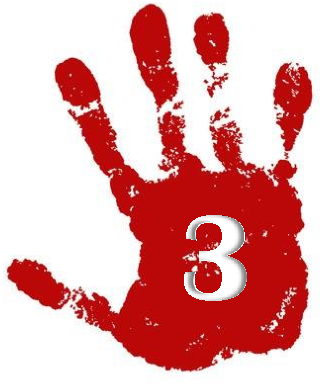
\includegraphics[width=0.05\linewidth]{./Figuras/Prevencao3.pdf}$}\label{sec:teste}%\icon{./Figuras/TrianguloCrime.pdf}


%Através dos escritos de Krafft-Ebing, o termo pedofilia foi criado no final do século XIX, quando a medicina por meio da psiquiatria começa a classificar os distúrbios mentais e os modos destoantes que deveriam ser banidos da sociedade. %https://www.riuni.unisul.br/bitstream/handle/12345/5994/tcc%20in%c3%a1cio%20-%20final.pdf?sequence=1&isAllowed=y

\section{Legislação}\label{sec:regras}%Normas, leis, regras, códigos

%O abuso sexual de crianças teve início na Antiguidade (desde 4 000 a.C.) e atualmente é um problema de saúde pública \cite{ribeiro2018programas}

%No Brasil, o período que antecedeu a Constituição Federal de 1988 (CF/88) foi determinantepara a mudança de paradigmas na área da garantia de direitos de crianças e adolescentes. A CF/88 foi um marco, na medida em que provocou uma substancial mudança no campo dos direitos humanos de crianças e adolescentes. O Brasil foi o primeiro país a promulgar um marco legal (Estatuto da Criança e do Adolescente), em consonância com a Convenção sobre os Direitos da Criança (1989). Estimase que o ECA tenha inspirado mais de 15 reformas legislativas, em especial na América Latina. %http://www.crianca.mppr.mp.br/arquivos/File/publi/sedh/08_2013_pnevsca.pdf 

%É dever constitucional da família, da sociedade e do Estado assegurar à criança e ao adolescente, com absoluta prioridade, o direito à vida, à saúde, à alimentação, à educação, ao lazer, à profissionalização, à cultura, à dignidade, ao respeito, à liberdade e à convivência familiar e comunitária. %https://www.riuni.unisul.br/bitstream/handle/12345/5994/tcc%20in%c3%a1cio%20-%20final.pdf?sequence=1&isAllowed=y

A elaboração de leis e normativas define um instrumento legal para a garantia dos direitos das crianças. Antes disso, no século XIX,
%A primeira monografia que descreve o abuso sexual infantil data de 1860 \cite{aded2006abuso}. Nesta época 
as cortes judiciais enxergavam os relatos de crianças que manifestavam o abuso sexual, como alegações fantasiosas ou mesmo mentirosas. A esperança das crianças de terem suas vozes devidamente ouvidas (e seu direitos assegurados) iria surgir apenas no século seguinte.
%https://bice.org/en/history-rights-child/
%https://childrightshub.org/en/history/

%“entre quase todos os povos antigos, tanto do Ocidente quanto do Oriente, os filhos durante a menoridade, não eram considerados sujeitos de direito, porém, servos da autoridade paterna.” (TAVARES apud OLIVEIRA, 2013).

%Mas, somente no final do século XIX, que a sociedade começou a mudar seu pensamento sobre a educação e tratamento destes indivíduos, o avanço era fraco, mas era um início, o surgimento da primeira concepção de criança. (OLIVEIRA, 2013).

No início do século XX, a sueca Ellen Key manifestou-se sobre o novo século denominando-o como `Século da Criança' \cite{sandin1999imagens, dos2015olhares, hayes2002children}. Este século marca a fundação da organização não governamental \textit{Save the Children}, responsável pela defesa dos direitos da criança no mundo. A fundação data de 1919, anos depois, em 1924 a fundadora da organização Eglantyne Jebb escreveu um documento que seria conhecido mundialmente como Declaração dos Direitos da Criança de Genebra ou Declaração de Genebra.

%http://www.un-documents.net/gdrc1924.htm [declaração de genebra]
%https://profuturo.education/en/2017/11/23/the-history-of-the-convention-of-the-rights-of-the-child/
A Declaração de Genebra estabelece cinco direitos fundamentais, os quais dão as crianças o direito de serem alimentadas, de serem ajudadas primeiro em caso de catástrofe, de serem escolarizadas, de serem bem tratadas e de serem protegidas contra qualquer forma de exploração. A Declaração dos Direitos da Criança de Genebra destaca-se na história como o primeiro documento internacional voltado a registrar e defender os direitos da criança. Em 1948 os direitos das crianças passaram a ser reconhecidos pela Declaração Universal dos Direitos Humanos, e pela Declaração dos Direitos da Criança adotada pela Assembleia Geral das Nações Unidas, em 1959 \cite{lelis2014fragmentaccao}. Anos depois em 1989, a Assembleia Geral da ONU adotou em suas normativas a Convenção sobre os Direitos da Criança, o qual tornou-se o instrumento de direitos humanos mais aceito na história, ratificado por 196 países. 
%http://www.revistas.usp.br/ran/article/view/124233/120991
%https://www.scielo.br/scielo.php?script=sci_arttext&pid=S0102-01881999000100002&lng=en&nrm=iso&tlng=pt
%https://www.scielo.br/pdf/rlae/v20n3/pt_a01v20n3.pdf
%http://www.publicadireito.com.br/artigos/?cod=99927ed3f11c0f36
%http://www.scj.pe.gov.br/scjpe/sites/all/themes/zentropy/pdf/producao_scj/CONSTRUINDOAERADOSDIREITOSHUMANOSporjoaocandido.pdf
%https://profuturo.education/en/2017/11/23/the-history-of-the-convention-of-the-rights-of-the-child/
%https://www.scielo.br/pdf/rpc/v33n4/a05v33n4.pdf
%https://www.tcd.ie/policy-institute/assets/pdf/BP9_Children_Hayes.pdf
%https://www.unicef.org/brazil/convencao-sobre-os-direitos-da-crianca

% Ano Internacional da Criança, em 1978

No Brasil, a história dos direitos das crianças e dos adolescentes começa em 1990, graças ao Estatuto da Criança e o Adolescente (ECA). O Estatuto é considerado um marco na defesa dos direitos da criança e do adolescente brasileiro \cite{lima2012direitos}. Os menores são protegidos pela legislação brasileira contra qualquer forma de negligência, discriminação, crueldade, opressão, violência e exploração. 

%Direito das crianças = 1924, pela Convenção de Genebra sobre os direitos da criança, estendida pela Convenção Internacional das Nações Unidas de 1959 e ratificada em 1990 pelos países signatários \cite{aded2006abuso} 

A legislação é um instrumento chave na luta contra o abuso sexual infantil. Os direitos estabelecidos juridicamente garante uma maior proteção aos menores. A tipificação de crimes contra as criança pode desencoragar certos agressores sexuais de praticarem seus delitos. Para os delitos já praticados, a legislação continua sendo um instrumento chave na luta contra o abuso sexual infantil, pois além de garantir tratamento as vítimas, assegura o encarceramento do criminoso sexual. Uma lei de 2014 por exemplo %(Lei 7220/14), 
torna hediondo o crime de exploração sexual de crianças e adolescentes, impedindo o condenado de obter anistia, graça ou indulto ou pagar fiança.

%Não falei sobre os códigos de conduta. 
%Não falei que a constituiçaõ de 1988 já estabelecia alguns direitos (e pelo que, algumas leis de anos anteriores também)
%https://books.google.com.br/books?hl=pt-BR&lr=&id=gHpmmREw-jwC&oi=fnd&pg=PA9&dq=conselho+tutelar&ots=csKHGcPPVh&sig=yxoM2HPB4x8ti8s9UU8EEkPOEBQ#v=onepage&q=conselho%20tutelar&f=false [capitulo 1 - evolução dos direitos]

\section{Ouvidorias e Canais de Denúncia}\label{sec:canais}

%``Foi criado o Disque-Denúncia Nacional de Abuso e Exploração Sexual Contra Crianças e Adolescentes – 0800-990500, sob a coordenação da Associação Brasileira Multidisciplinar de Proteção à Criança e ao Adolescente (Abrapia), através de convênio com oDepartamento da Criança e do Adolescente do Ministério da Justiça.''
%https://www.gov.br/mdh/pt-br/acesso-a-informacao/ouvidoria/Disque_Direitos_Humanos.pdf

%``O enfrentamento do violência sexual no âmbito dos \textbf{órgãos públicos estatais e federais ocorre em forma de campanhas de mobilização da cidadania}, através dos meios presentes de comunicação. Nas cidades, essas campanhas chegam através de chamadas, em emissoras de televisão, pela distribuição de panfletos e exposição de mensagens, de propagandas escritas, nas ruas, ou breves alertas nas emissoras de rádio. Também pela divulgação do \textbf{número telefônico 181} , que é reservado para denúncias dessa prática delitiva.'' ... ``enfrentamento da prática de abuso sexual que exige a presença de agentes vinculados ao Sistema Único de Assistência Social-SUAS, ao Sistema Único de Saúde-SUS, ao Sistema Nacional de Educação e às unidades locais de Segurança Pública'' [o artigo tambem falo do SIPIA-CT Web, CREAS e do CRAS] \cite{caccia2014conselheiros}

%O avanço da legislação trouxe ferramentas não só para combater e coibir esta violência, clareando o limite entre criança e adulto, mas para possibilitar a criação de medidas sócio-educativas, protetivas e preventivas frente aos danos psicológicos que muitas vezes podem ser irreversíveis, além dos efeitos físicos e sexuais. Nosso país foi o primeiro país a promulgar um marco legal com a criação do Estatuto da Criança e do Adolescente (ECA), \cite{tonello2018pedofilia}

\begin{wrapfigure}[36]{r}{4.3cm}%pulando 36 linhas
  \vspace{-20pt}
  \caption{\label{fig:Canais}Ouvidoria Infantil\vspace{5pt}}

  \subfloat[Brasil\label{fig:Brasil}\vspace{-5pt}]{
\includegraphics[width=\linewidth]{./Figuras/Ouvidorias/100-Brasil.png}}\vspace{-3pt}
  \\
  \subfloat[Argentina\label{fig:Argentina}\vspace{-5pt}]{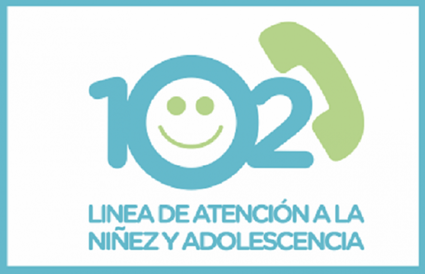
\includegraphics[width=\linewidth]{./Figuras/Ouvidorias/102-Argentina.png}}\vspace{-3pt}
  \\
  \subfloat[Vietnã\label{fig:Vietna}\vspace{-5pt}]{
\includegraphics[width=\linewidth]{./Figuras/Ouvidorias/111-Vietna.png}}\vspace{-3pt}
  \\
  \subfloat[França\label{fig:Franca}\vspace{-5pt}]{
\includegraphics[width=\linewidth]{./Figuras/Ouvidorias/119-Franca.png}}\vspace{-3pt}
  \\
  \subfloat[Aruba\label{fig:Aruba}\vspace{-5pt}]{
\includegraphics[width=\linewidth]{./Figuras/Ouvidorias/131-Aruba.png}}\vspace{-3pt}
  \\
  \subfloat[Japão\label{fig:Japao}\vspace{-5pt}]{
\includegraphics[width=\linewidth]{./Figuras/Ouvidorias/189-Japao.png}}\vspace{-3pt}
  \\
  \subfloat[Índia\label{fig:India}\vspace{-5pt}]{
\includegraphics[width=\linewidth]{./Figuras/Ouvidorias/1098-India.png}}\vspace{-3pt}
  \\
  \subfloat[Tailândia\label{fig:Tailandia}\vspace{-5pt}]{
\includegraphics[width=\linewidth]{./Figuras/Ouvidorias/1387-Thailandia.png}}
  %\begin{center}
  %  
\includegraphics[width=\linewidth]{./Figuras/Ouvidorias/100-Brasil.png}
  %\end{center}
  %\begin{center}
  %  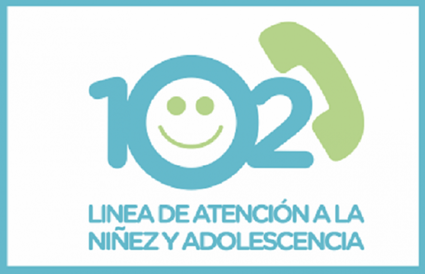
\includegraphics[width=\linewidth]{./Figuras/Ouvidorias/102-Argentina.png}
  %\end{center}
  %\begin{center}
  %  
\includegraphics[width=\linewidth]{./Figuras/Ouvidorias/131-Aruba.png}
  %\end{center}
  %\begin{center}
  %  
\includegraphics[width=\linewidth]{./Figuras/Ouvidorias/111-Vietna.png}
  %\end{center}
  %\begin{center}
  %  
\includegraphics[width=\linewidth]{./Figuras/Ouvidorias/189-Japao.png}
  %\end{center}
  %\begin{center}
  %  
\includegraphics[width=\linewidth]{./Figuras/Ouvidorias/1098-India.png}
  %\end{center}
  %\begin{center}
  %  
\includegraphics[width=\linewidth]{./Figuras/Ouvidorias/1387-Thailandia.png}
  %\end{center}
  %\begin{center}
  %  
\includegraphics[width=\linewidth]{./Figuras/Ouvidorias/119-Franca.png}
  %\end{center}
  \vspace{-8pt}
  \legend{Fonte: \cite{linhas2017}}%eu paguei outros nao citados aqui, como fazer a referencia?
  %india (mas não governamental)
\end{wrapfigure}

%https://www.argentina.gob.ar/justicia/violencia-familiar-sexual [A argentina atende também por WhatsApp = Mensageiros Instantaneos (além do telefone 137 e do email vicontravio@jus.gov.ar)]

Os canais de denúncia são uma estratégia relevante no combate a violência sexual infantil. Os meios de comunicação para delação servem de alicerce para garantir os direitos legalmente estabelecidos das crianças e dos adolescentes. Entre os meios de denúncia mais amplamente presentes pelo mundo estão as linhas telefonicas. A \autoref{fig:Canais} elenca as principais ouvidorias telefonicas de alguns países.

%Canais não presenciais de atendimento (ao cidadão)

Os números telefonicos da \autoref{fig:Canais} demonstram a procupação dos países em garantir um canal seguro de comunicação para crianças em situação e risco. A depender do país, cada canal de comunicação pode aceitar outras formas de denúncia, além da violência infantil. No caso do Brasil, o Disque 100 (Figura\autoref{fig:Brasil}), além de receber denúncias contra crianças e adolescentes, também recebe denúncias de outros grupos vulneráveis como idosos e deficientes. Os meios de denúncia veem no intuito de mitigar as lacunas deixadas pelas políticas públicas no que diz respeito a fiscalização.

Os canais telefônicos são instrumentos de denúncia a distância confiáveis e acessíveis \cite{linhas2017}. A penetrância dos dispositivos móveis no Brasil, torna este intrumento ainda mais poderoso no combate a violência infantil, uma vez que a quantidade de dispositivos móvies operantes no país ultrapassa a própria população brasileira. Além das denúncias por ouvidorias telefonicas, as denuncia podem ser realizadas por correio eletrônico, aplicativos e portais governamentais. As denúncias no Brasil podem ser realizadas de forma totalmente gratuita durante toda a semana 24 horas por dia (incluindo sábados, domingos e feriados).

O processo de denúncia se aplica tanto para crimes tentados quanto para crimes praticados. Deste modo, amplia-se a possibilidade de garantir a segurança e bem estar das crianças antes ou após a violência, bastando para isso, um meio de comunicação e um número telefônico. Neste sentido, cabe destacar os números de cada país são válidos apenas em carater nacional, a linha internacional de denúncia do Brasil é: +55 (61) 3212-8400.

%Não falei do AloAloBrasil (Alo123), nem do SaferNet.


%As linhas de atendimento infantil estão no cruzamento crítico, onde crianças e jovens encontram seu caminho para a proteção e os cuidados prestados pelos sistemas de proteção infantil; eles são fontes confiáveis e acessíveis de ajuda e apoio a crianças e jovens e de encaminhamento para o sistema de proteção infantil, incluindo a aplicação da lei, se necessário\cite{linhas2017}

%https://www.unicef.org/protection/files/LEAP_report_CHI_and_UNICEF_(final).pdf \cite{linhas2017}
%https://www.police.sa.gov.au/your-safety/child-safety
%https://www.childhelplineinternational.org/child-helplines/child-helpline-network/
%\footnote{ \url{https://www.childhelplineinternational.org/child-helplines/child-helpline-network/}}


%colocar as policias antes...
\section{Propagandas}\label{sec:propagandas}

As propagandas são um mecanismo chave no combate ao abuso sexual infantil. Os meios de divulgação ajudam na dispersão do conhecimento e na conscientização da população. Os programas de conscientização da população são largamento conhecidos por auxiliarem suas respectivas lutas. %seja em capampanhas de vacinação ou em campanhas de combate a mosquitos transmissores de doenças. 
No caso do abuso sexual infantil, as propagandas auxiliam as crianças sobre seus direitos ensinando-as e encorajando-as a realizarem denúncias. Um exemplo de propaganda neste estilo é apresentado tanto na \autoref{fig:adulto} quanto na \autoref{fig:crianca}.

\begin{figure}[htb]
  %\caption{\label{fig:propagandas}Propaganda}
  \begin{center}
  \begin{minipage}[t]{0.5\textwidth}
    \caption{\label{fig:adulto}Propaganda na visão do Adulto}
    \vspace{0.1cm}
    \centering
    \frame{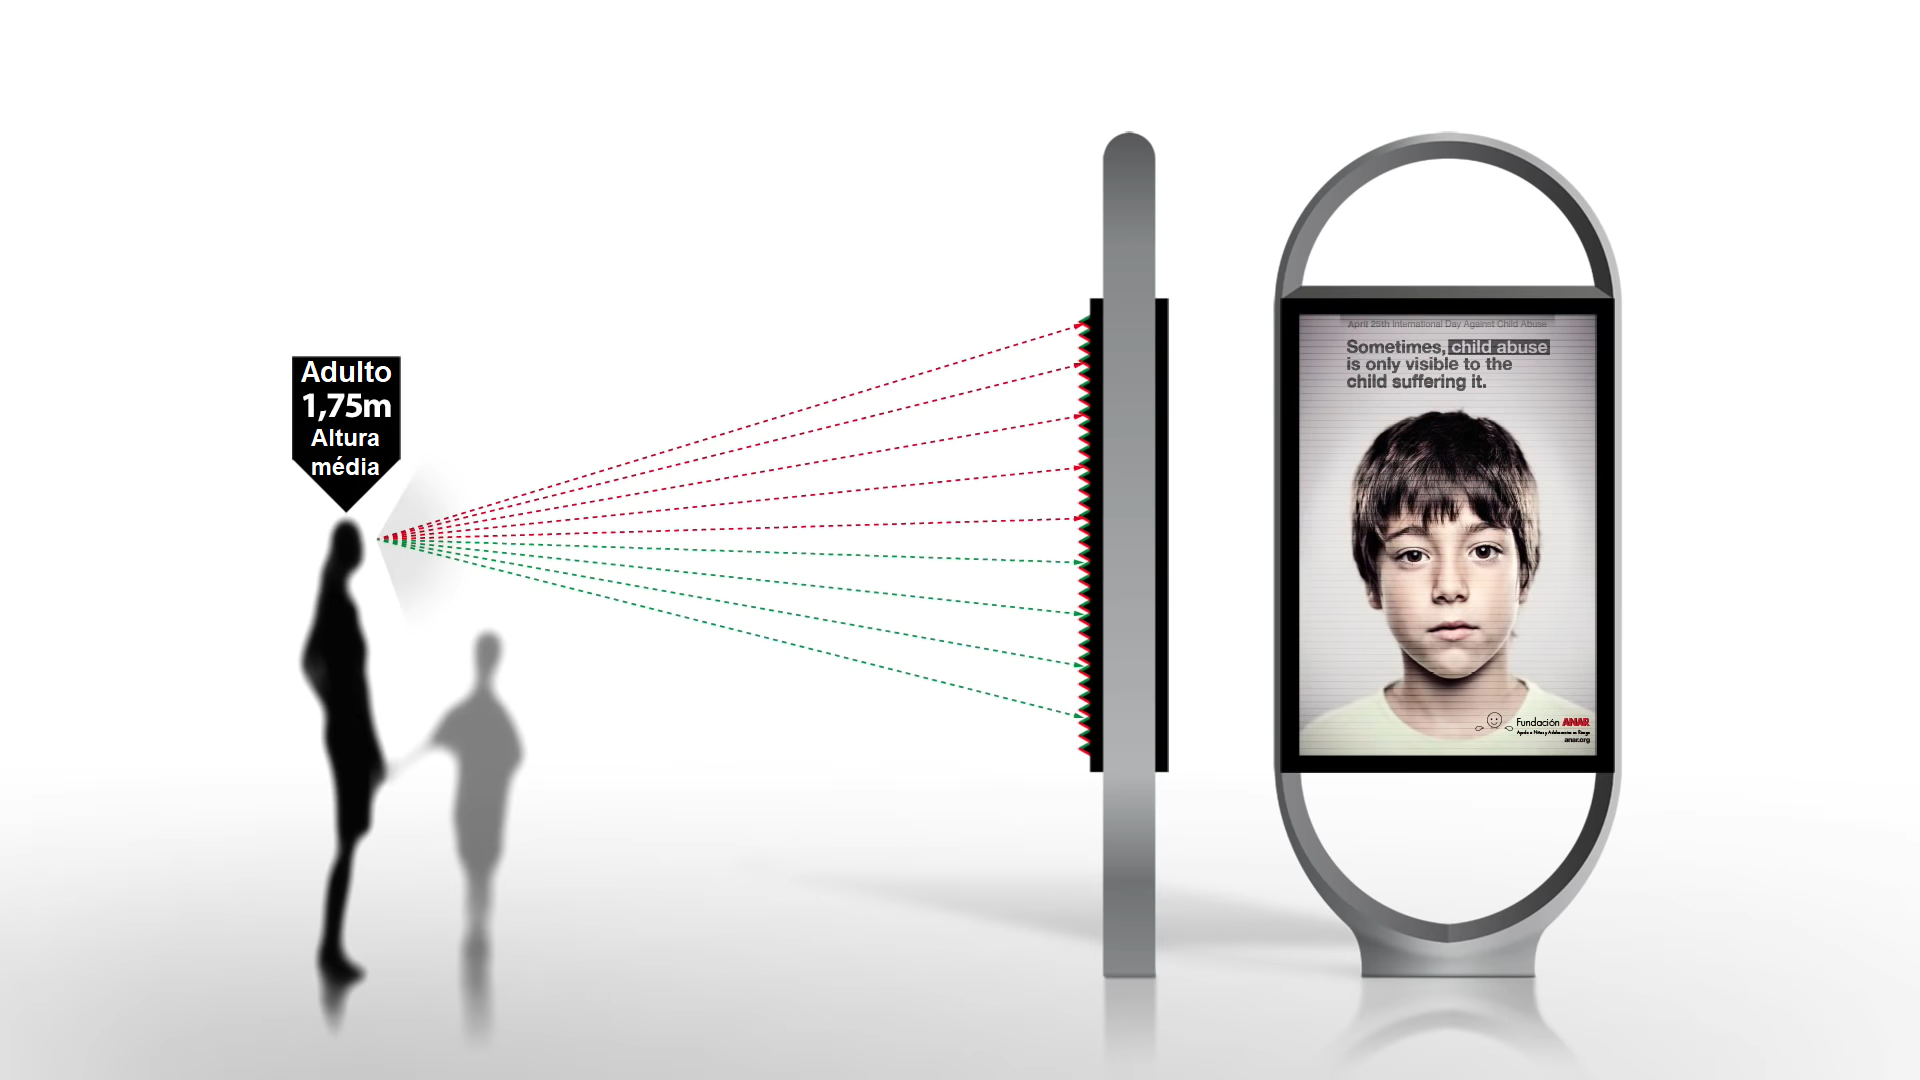
\includegraphics[width=\linewidth]{./Figuras/Propagandas/Propaganda-Adulto.png}}      
\end{minipage}%
~ 
\begin{minipage}[t]{0.5\textwidth}
    \caption{\label{fig:crianca}Propaganda na visão da Criança}
    \vspace{0.1cm}
    \centering
    \frame{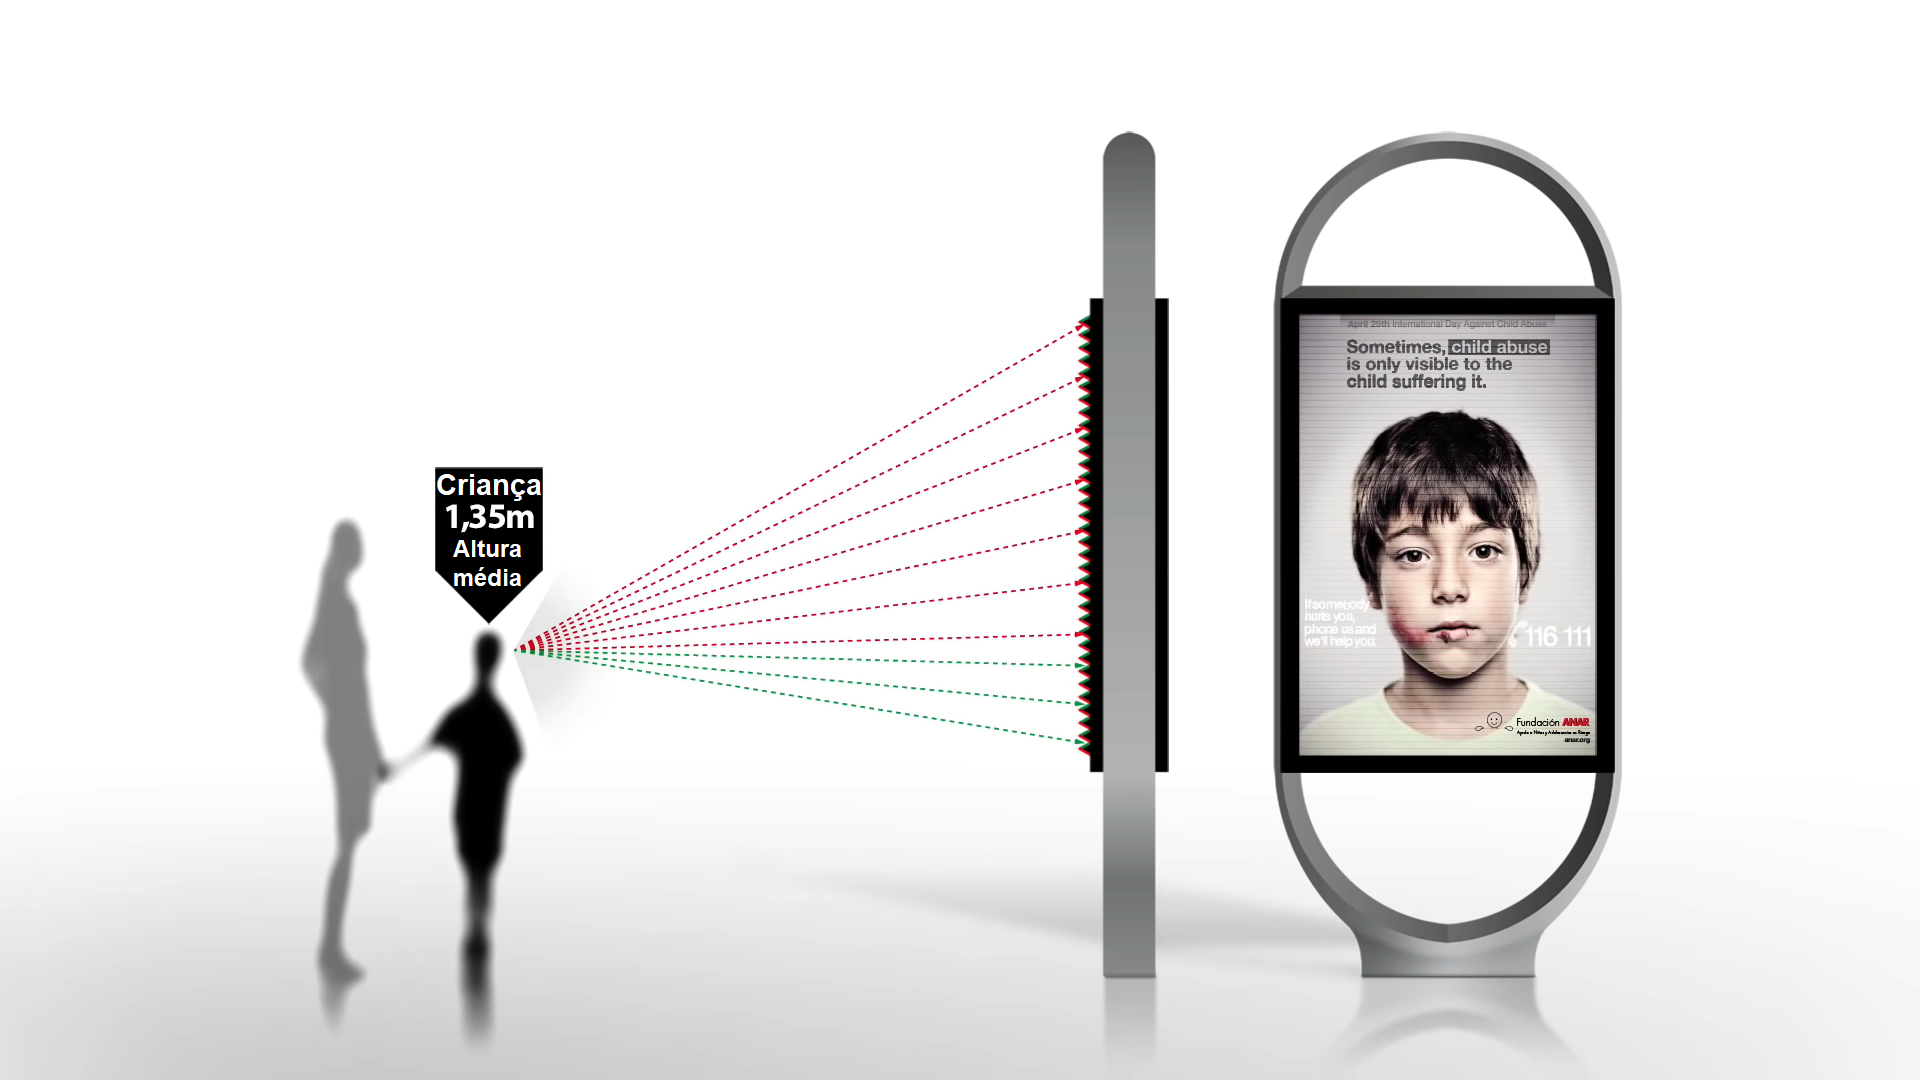
\includegraphics[width=\linewidth]{./Figuras/Propagandas/Propaganda-Crianca.png}}
\end{minipage}

	\end{center}
  \legend{Fonte: adaptado de ....}
%https://www.youtube.com/watch?v=6zoCDyQSH0o   - Anar Foundation
%https://www.youtube.com/watch?v=N0h1mgpn95s&feature=emb_title [trocar, esse é o original]
\end{figure}
%"Si alguien te hace daño llámanos y te ayudaremos"

A \autoref{fig:adulto} e a \autoref{fig:crianca} apresentam a mesma propaganda, porém vista de ângulos diferentes. A propaganda parte da concepção de que muitas crianças violentadas transitam pelas ruas com seus próprios agressores. Agressores estes, que para não serem encarcerados garantem o desconhecimento da criança sobre os meios de denúncia relativos ao crime cometido. A propaganda então, baseada sob estes princípios, apresenta uma mensagem visível apenas apartir do ângulo de visão da altura média de uma criança (1,35 metros). A mensagem, dentre outras informações, apresenta aos menores um número telefónico, o qual permite um canal de ajuda e socorro as crianças vítimas de violência. 

As propagandas auxiliam na divulgação de informações, as quais capacitam as pessoas a reconhecerem o problema e a reagirem adquadamente ao problema. Os meios de comunicação são os mais variados, podendo ir desde comerciais no rádio, na televisão ou na internet \cite{martinez2011prevencion}. Além disso, excelentes meios de divulgação são cartazes, panfletos, cartilhas e campanhas governamentais \cite{mendelson2015parent}.


%``Existe una gran variedad de opciones metodologicas al alcance de los usuarios. Dentre de estas, las mas utilizadas han sido los \textbf{materiales impresos, los videos o materiales audiovisuales, las charlas, las representaciones teatrales y el role playing}'' (corrigir erros do espanhol) [Esse artigo é bom, pois fala dos toque bons, toque ruins, partes íntimas, etc] ... ``el abusador impone a el nino ley de silencio (segredo)'' ... ``los programas deberian poner el acento en transmitir a los ninos la importancia de divulgar el abuso y no en pedirles que se nieguen y sean capaces de deternerlo'' [LEMBRA DO JOGO TRIALHA DA PROTEÇÃO, ao completar a criança recebe o título de 'PROTEGIDO'] \cite{martinez2011prevencion} 


\section{Atendimento Hospitalar}\label{sec:hospital}

Os atendimentos hospitalares são procedimentos poderosos no combate aos maus tratos contra as crianças. O profissional de saúde surge como um sujeito ativo, no sentido de identificar abusos e denunciá-los, conforme ordenada a legislação brasileira \cite{costa2019maus}. Inúmeros jornais e portais de notícias já relataram inclusive o diagnóstico de violência sexual infantil em laudos médicos\footnote{Redação de Notícias Catve.com (28/12/2018): \url{https://catve.com/noticia/9/238135/menina-de-11-anos-e-internada-com-dores-abdominais-e-medico-descobre-gravidez}}\footnote{Portal de Notícias G1 (08/08/2018): \url{https://g1.globo.com/ro/ji-parana-regiao-central/noticia/2018/08/08/mae-leva-filha-de-5-anos-ao-pediatra-e-descobre-que-menina-foi-estuprada-em-ro.ghtml}}\footnote{Jornal Metropóles (07/06/2016): \url{https://www.metropoles.com/distrito-federal/seguranca-df/medico-denuncia-estupro-de-menina-de-11-anos-em-festa-de-escola-no-df}}\footnote{Rede Jornalística A Gazeta (03/11/2017): \url{https://www.gazetaonline.com.br/noticias/policia/2017/11/menino-contrai-sifilis-e-familia-descobre-abuso-sexual-1014106068.html}}\footnote{Portal de Notícias G1 (26/08/2015): \url{http://g1.globo.com/sao-paulo/itapetininga-regiao/noticia/2015/08/mae-descobre-que-filho-foi-estuprado-apos-dentista-achar-doenca-na-boca.html}}\footnote{Portal de Notícias G1 (23/04/2013): \url{http://g1.globo.com/sp/bauru-marilia/noticia/2013/04/exame-aponta-que-menina-de-3-anos-sofreu-abuso-sexual-em-bauru-sp.html}}.%\footnote{Correrio do Estado (31/07/2019): \url{https://www.correiodoestado.com.br/cidades/exame-aponta-doenca-e-tia-descobre-estupro-de-criancas/357839/}}\footnote{Portal G1 (08/08/2019): \url{https://g1.globo.com/sp/sao-jose-do-rio-preto-aracatuba/noticia/2019/08/08/pais-tiram-crianca-de-hospital-antes-de-alta-apos-medico-suspeitar-de-sinais-de-abuso-sexual.ghtml}}.

%https://g1.globo.com/bahia/noticia/crianca-de-oito-anos-morre-por-insuficiencia-respiratoria-apos-estupro.ghtml [mórbido demais para citar, eu acho]

%https://www.google.com/url?sa=t&rct=j&q=&esrc=s&source=web&cd=8&cad=rja&uact=8&ved=2ahUKEwia2sGezbHpAhUND7kGHcVjDx4QFjAHegQICBAB&url=https%3A%2F%2Fwww.radiocacula.com.br%2Fnoticias%2Fcidades%2Fmenina-de-4-anos-morre-medico-descobre-estupro-e-pai-e-o-suspeito&usg=AOvVaw0k64eNQ83eicbnl4eJGl55 [mórbido demais para citar, eu acho]

A literatura médica comenta sobre a dificuldade em constatar sinais de violência infantil em alguns casos. Em certas circunstância se exige do médico muito mais perspicácia e experiência profissional \cite{de2012violencia}. Devido a complexidade no diagnósitico de alguns episódios de abuso, guias clínicos foram desenvolvidos como o Guia Clínico da Organização Mundial da Saúde \cite{world2017responding}. Os relatórios e guias médicos são capazes de ajudar os profissionais de saúde a identificar mais facilmente sinais de abuso acometidos contra a criança e contra o adolescente \cite{Christian1}.

%``This guideline aims to provide evidence-based recommendations for quality clinical care for children and adolescents who have, or may have, been subjected to sexual abuse, in order to mitigate the negative health consequences and improve their well-being. The objectives are to support health-care providers to provide quality, immediate and long-term clinical care and to apply ethical, human-rights-based and trauma-informed good practices in the provision of such care. Where relevant for provision of clinical care and where there is supporting evidence, sex-based differences and gender-based inequalities are flagged.''\cite{world2017responding}

%``the report can help primary care pediatricians learn clinical clues to the diagosis of abuse and undertand specific injuries of concern, appropriate diagnostic testes and considerations, and legal requirements related to mandated reporting of suspected abuse'' \cite{Christian1}

Os guias e relatórios médicos ajudam tanto no diagnósitico, quanto na procedências dos tramites legais. Nos casos agudos de violência sexual, com menos de 72h do ocorrido, as medidas legais já devem acompanhar toda a assistência inicial de diagnóstico e tratamento. Nos casos crônicos e repetitivos, sem grandes lesões visíveis, será fundamental o registro de anamnese, histórico familiar e dados de exame físico. Para fins de processo judicial e a necessária comprovação da agressão, bem como para confecção de exames que levem à identificação do agressor, é preciso que os responsáveis façam um boletim de ocorrência em delegacia de policia, que requisitará o laudo pericial do Instituto Médico Legal \cite{de2012violencia}. 

O atendimento hospitalar adiciona mais uma camada de defesa no enfretamento a violência sexual infantil. Embora os abusos só possam ser diagnósticados após sua ocorrência, a defesa médica ainda se faz válida para diminuir a reincidência dos eventos abusivos, seja em um exame de rotina ou qualquer outra forma de atendimento \cite{costa2019maus}.

%``No atendimento do consultório odontológico o cirurgião-dentista pode encontrar crianças com lesões características de violência física, seja em um exame de rotina ou qualquer outra forma de atendimento''\cite{costa2019maus}

%\cite{christian2015evaluation}

%O método clínico, composto pela anamnese e o exame físico e auxiliado por exames complementares, é o maior arsenal que o médico dispõe para o diagnóstico de maus tratos ou violência infantil \cite{de2012violencia}.

%http://www2.fm.usp.br/gdc/docs/iof_152_5-violencia.pdf [LER]
%https://repositorio.unb.br/bitstream/10482/2302/1/Sonia%20Fortes%20do%20Prado.pdf



\section{Centros de Tratamento às Vítimas}\label{sec:centros}

%Resultados da pesquisa Trecho da Web em destaque O Centro de Referência às Vítimas de Violência (CRVV) é um serviço do Município, em parceria com o Governo Federal, criado para prestar informações e orientações às vítimas de violações de direitos, abuso de autoridade, exploração sexual e qualquer tipo de discriminação.

Os centros de tratamento estabelecem uma poderosa estratégia de enfretamento ao maltrato infantil. No Brasil, o tratamento e recuperação da criança vítima de violência pode ser executado pelo Conselho Tutelar. Os Conselhos Tutelares estão para a violência sexual infantil e adolescente, como as equipes de resgate estão para os primeiros socorros \cite{caccia2014conselheiros}.

%Art. 131. O Conselho Tutelar é órgão permanente e autônomo, não jurisdicional, encarregado pela sociedade de zelar pelo cumprimento dos direitos da criança e do adolescente, definidos nesta Lei (ECA). 

O Conselho Tutelar é um órgão permanente e autônomo, não jurisdicional, encarregado de zelar pelo cumprimento dos direitos da criança e do adolescente \cite{saude2002notificacao}. Além do Conselhor Tutelar, a nível nacional ainda é possível citar o Centro de Referência Especializado de Assistência Social (Creas), responsável pelo acolhimento e pelo atendimento a famílias e indivíduos em situação de risco pessoal e social, por violência, abuso e exploração sexual, ocorrência de abandono, maus-tratos físicos e/ou psíquicos, cumprimento de medidas socioeducativas, situação de rua e de trabalho infantil, entre outras situações de violação dos direitos.

Os centros de tratamento não são uma exclusividade apenas do Brasil. Estratégias do gênero podem ser encontradas em várias países pelo globo, como: Madri\footnote{ Centro especializado de Intervención en abuso sexual infantil (CIASI): \url{http://edicion.comunidad.madrid/servicios/asuntos-sociales/intervencion-abuso-sexual-infantil}}, Equador\footnote{Centro Integral de la Niñez y Adolescencia (CENIT): \url{http://cenitecuador.org/}} %que é uma organização sem fins lucrativos
e Argentinha\footnote{Centro Integral Especializado en Niñez y Adolescencia (CIENA): \url{https://www.buenosaires.gob.ar/desarrollohumanoyhabitat/mujer/hogares-y-centros-integrales-de-la-mujer/asistencia-al-maltrato-infantil}}. Embora os objetivos dos centros sejam similares, a estrutura organizacional e operacional pode variar bastante de centro para centro. No caso do Brasil, a lei obriga que exista pelo menos um Conselho Tutelar por município composto de pelo menos cinco membros com idoneidade moral escolhidos pela comunidade local. %https://www.mpdft.mp.br/portal/pdf/unidades/promotorias/pdij/Conselhos/guia_conselheirotutelar11.pdf

O Conselho Tutelar e demais centros de tratamento veem na perspectiva de atuar diante dos maus-tratos sem se limitar ao tratamento médico dos traumas e lesões resultantes desses problemas \cite{brasil2002notificaccao}. A implementação de centros do gênero estabelece um grande aliado na proteção dos direitos da infância e da juventude e a sua implementação no país é de extrema importância para o enfrentamento à violência contra crianças e adolescentes. %https://www.childhood.org.br/conquistas-do-eca-criacao-do-conselho-tutelar
O Conselho Tutelar não presta o atendimento direto, mas atua de forma que ele se viabilize em casos concretos de ameaça ou violação de direitos. O ECA prevê que os casos de suspeita ou confirmação de maus-tratos contra criança ou adolescente serão obrigatoriamente comunicados ao Conselho Tutelar da respectiva localidade, sem prejuízo de outras providências legais.

%Centros de Referências em Assistência Social – CREAS e Centros de Atendimento Psicossocial – CAPS, esses centros são acionados para atendimento psicossocial e de assistência social e também para encaminhamentos de casos de drogadição.


%``Abuso sexual: consiste em todo ato ou jogo sexual, relação heterossexual ou homossexual cujo agressor está em estágio de desenvolvimento psicossexual mais adiantado que a criança ou o adolescente. Tem por intenção estimulá-la sexualmente ou utilizá-la para obter satisfação sexual. Apresenta-se sobre a forma de práticas eróticas e sexuais impostas à criança ou ao adolescente pela violência física, ameaças ou indução de sua vontade. Esse fenômeno violento pode variar desde atos em que não se produz o contato sexual (voyerismo, exibicionismo, produção de fotos), até diferentes tipos de ações que incluem contato sexual sem ou com penetração. Engloba ainda a situação de exploração sexual visando lucros como é o caso da prostituição e da pornografia.'' \cite{saude2002notificacao} [Essa referencia também explica um pouco sobre o conselho Tutelar]


\section{Departamentos Policiais}\label{sec:dp}

As delegacias especializadas são um bom artifício de confronto a violência sexual infantil. A Delegacia de Proteção à Criança e Adolescente (DPCA) é competente para fiscalizar, investigar e instaurar inquérito e procedimentos policiais nos casos de infração penal praticada contra crianças e adolescentes. Isso significa que a DPCA é responsável por crimes em que as crianças e adolescentes são as vítimas e não autores do delito. Além desta função, a DPCA também desenvolve estratégias de repressão continuadas em qualquer local, público ou privado, como forma de interromper o ciclo de impunidades dos agressores \cite{rodrigues2014}. %Toda prática de violência contra criança ou adolescente deve ser denunciada nesta delegacia especializada. Não é necessário se identificar para comunicar algum crime 

As delegacias especializadas são consideradas determinantes no processo de visibilidade da violência sexual contra crianças e adolescentes \cite{plano2013}. Não atoa, sua presença se alastra por outros países ao redor do mundo, como por exemplo: Colombia\footnote{Delegacia da Infância e Adolescência (Policía de Protección a la Infancia y Adolescencia)}, Índia\footnote{Special Juvenile Police Units (SJPU)} e França\footnote{Brigade de protection des mineurs}.
%BRASIL: Delegacia de Proteção à Infância e Adolescência
%Colombia: 
%India? : Special Juvenile Police Units(SJPU) %http://www.wcddel.in/Guidelines[1].pdf
%França: Brigade de protection des mineurs: %https://www.prefecturedepolice.interieur.gouv.fr/Nous-connaitre/Services-et-missions/Missions-de-police/La-direction-regionale-de-la-police-judiciaire/La-brigade-de-protection-des-mineurs
Não há uma diretriz operacional única entre as delegacias especializadas, nem mesmo a nível nacional. No Brasil, algumas delegacias ficam abertas 24 horas por dia todos os dias da semana, enquanto outras operam apenas nos dias úteis e em horário comercial. E mesmo as abertas 24 horas não possuem uma equipe multidisciplinar de plantão, contando com apenas os funcionários essênciais para o registro da ocorrência como agentes, escrivães e delegado \cite{novo2016}. 

Boa parte das iniciativas de criação de DPCAs ainda são muito recentes, ressaltando-se a carência tanto de legislação específica quanto de pesquisas e material especializado publicados sobre elas \cite{novo2016}. Isso ajuda a explicar melhor as divergências encontras entre as delegacias no que diz respeito a presença ou não de carceragem, brinquedoteca e salas de atendimento psicológico. 
%meio que todas tem briquedoteca, mas é tipo um chuncho
Em adendo, algumas Delegacias relataram convênios com hospitais, universidades e Organizações Não Governamentais.

As delegacias especializadas integram o Sistema de Garantias dos Direitos da Criança e do Adolescente. Essas delegacias ainda podem se dividir entre as voltadas para o atendimento às vítimas ou voltadas para a lidar com os infratores, havendo ainda aquelas que conjugam as duas funções em um mesmo órgão. A efetividade dos mecanismos de denúncia e notificação garante a possibilidade não apenas de atendimento às vítimas, mas também de responsabilização e tratamento dos agressores, evitando a impunidade e o ciclo repetitivo da violência \cite{novo2016}.

%DPCA – DELEGACIA DE PROTEÇÃO À CRIANÇA E AO ADOLESCENTE
%DPAI - Delegacia de Polícia do Adolescente e outras

%https://www.camara.leg.br/noticias/604913-comissao-aprova-notificacao-obrigatoria-de-maus-tratos-e-automutilacao-de-criancas/ [NOTIFICACAO OBRIGATORIA]

%O Sistema de Garantia dos Direitos da Criança e do Adolescente compreende oscentros de defesas, as delegacias especializadas, a vara da infância e juventude, aspromotorias da infância e juventude, conselho tutelar, conselho de direitos, dentre outros. Ésalutar apresentar informações alusivas a estas instituições, já que podem ser acionadasquando da denúncia de abuso sexual \cite{rodrigues2014}.


\section{Operações Policiais}\label{sec:op}

As operações policiais são excelentes alternativas na luta contra o abuso e a exploração sexual infantil. No Brasil e no mundo as operações são responsáveis pela busca e apreensão de inúmeros criminosos sexuais, o que acaba por mitigar a reincidência do crime por parte destes agressores. 

A literatura relata a Operação Carrossel (2007) como o primeiro esforço policial internacional a combater a pornografia infantil na internet \cite{lowenkron2014all}. Todavia, há registros anteriores que relatam a mesma abragência policial internacional, como a Operação Catedral (1998) objetivada também no combate a pornografia infantil na internet \cite{Barrot2008, jesus2006anti}. É importante destacar que isto não se trata necessariamente de uma contradição literária, a Operação Darknet (2014) também é descrita como pioneira no combate a distribuição de material pornografico infanto-juvenil na internet, contudo o pionerismo desta, configura-se pela metodologia de investigação e pelas ferramentas para identificar usuários criminosos na DeepWeb \cite{tonello2018pedofilia}. Ou seja, cada operação pode ser classificada como pioneira com base em seus contextos específicos. 

%A Agência de Notícias da Polícia Federal apresenta dados sobre a operação Darknet, investigação pioneira, que objetivou combater uma rede de distribuição de pornografia infanto-juvenil na Darkweb, foi deflagrada pela polícia Federal em 2014 e 2016. Na primeira fase foram cumpridos 93 mandados de busca e na segunda fase 70. A Polícia Federal antecipou o cumprimento de 7 ordens judiciais para evitar o possível abuso sexual de crianças. Desde a primeira fase da Operação Darknet (2014), a Polícia Federal desenvolve metodologia de investigação e ferramentas para identificar usuários da DarkWeb, considerado um meio seguro de divulgação de conteúdos variados de forma anônima. A arquitetura desse ambiente impossibilita a identificação do ponto de acesso (IP), ocultando o real usuário que acessa a rede. Poucas polícias no mundo obtiveram êxito em investigações na Darkweb, como o FBI, a Scotland Yard e a Polícia Federal Australiana \cite{tonello2018pedofilia}.

%depois de seis meses de uma ação integrada em prol do combate a crimes de exploração sexual contra crianças, chamada de Operação Luz na Infância 2, foram presas, em maio de 2018, 21 pessoas, incluindo uma criança, na posse de material com conteúdo de exploração sexual infanto-juvenil. Em Porto Alegre, foram oito prisões, duas em Santa Maria, duas em Cachoeirinha e duas em Novo Hamburgo, além de prisões efetuadas em Alvorada, Pelotas, Panambi, Taquara, Canoas, Sapucaia, São Leopoldo e Viamão. Também foram apreendidos diversos computadores, notebooks, HDs externos, pendrives e outros dispositivos de armazenamento que continham material referente a crimes de abuso e exploração sexual infanto-juveni \cite{tonello2018pedofilia}.

No Brasil, o Ministério da Justiça considera a Operação Luz na Infância (2017) como a maior operação do gênero no Brasil e na América Latina. Isto, pois a operação é um conglomerado de vários países e instituições \cite{souza2018sabemos}. Entre os países estão: Brasil, Chile, El Salvador, Equador, Estados Unidos, Panamá e Paraguay. A Operação já teve mais de cinco fases apreendendo um volume total de dados que ultrapassa os três terabytes, além da pisão de mais de 500 indivíduos. 

%A Polícia Federal já deflagrou algumas operações que tinham como objetivo combater a pedofilia na internet. As primeiras foram as intituladas como Carrossel I (2007) e Carrossel II (2008). E em outubro de 2017, a Operação Luz na Infância, que foi considerada pelo Ministério da Justiça, a maior operação que houve no Brasil e na América Latina, de acordo com a matéria do jornal a Folha (2017). \cite{souza2018sabemos}

As operações policiais são políticas públicas de segurança que estão fundamentadas e baseadas nos limites da legislação e da jurisdição de suas nações, reguardados os acordos internacionais. Dito isso, é notória a dependência que as operações policiais possuem com o âmbito jurídico. Se não há tipificação legal do crime, então não a crime a ser reprimido. Por tal razão que a sansão de decretos e a criação de leis neste contexto se fazem fundamentais para o fortalecimento das operações policiais. 

%Em 8 de maio de 2017, foi sancionada a Lei de Nº 13.441 que altera a lei do ECA e prevê a infiltração de agentes de polícia na internet com o fim de investigar crimes contra a dignidade sexual de crianças e adolescentes (BRASIL, 2017). \cite{souza2018sabemos}

%Operação Luz na Infância (2018) (7 países) \cite{souza2018sabemos}
%Operação Tapete Persa (2010) \cite{da2012bibliotecas} \cite{barros2014pedofilia}
%Operação Darknet (2014) %http://www.mpf.mp.br/rs/sala-de-imprensa/docs/outros-documentos/operacao-darknet
%Operação Carrossel (2007) \cite{souza2018sabemos}
%Operação Alanis (2016)

%Operation Netsafe (2017) Reino Unido (wales) %https://www.gwent.police.uk/en/newsroom/operations-campaigns/operation-netsafe/ %https://www.south-wales.police.uk/en/advice/child-sexual-exploitation-cse/operation-net-safe-tackling-online-child-sexual-abuse-and-exploitation/

%Operação Atelier (2014) EUROPOL %https://www.europol.europa.eu/activities-services/europol-in-action/operations/operation-atelier

%OPERATION RESCUE (2011) EUROPOL %https://www.europol.europa.eu/activities-services/europol-in-action/operations/operation-rescue

%OPERATION ATLANTIC (2010) EUROPOL %https://www.europol.europa.eu/activities-services/europol-in-action/operations/operation-atlantic

%OPERATION ICARUS (2011) EUROPOL %https://www.europol.europa.eu/activities-services/europol-in-action/operations/operation-icarus

%OPERATION ARCHIMEDES = EUROPOL + INTERPOL

%Operação Catedral (1998) (12 países) \cite{jesus2006anti} [aqui fala da operação e como legislar sobre um site que opera em um país mas está hospedado em outro]


%http://www.pf.gov.br/agencia/noticias/2014/10/pf-combate-a-disseminacao-de-pornografia-infantil-pela-deep-web-no-rs

A dependência juridica das operações políciais pode ser uma barreira a ser enfrentada no combate a violência sexual infantil. De nada adianta uma operação contra o abuso de crianças em um país que premite legalmente o casamento infantil. Além da barreira jurídica, as estratégias policiais sofrem do mesmo mal dos atendimentos hospitalares, uma vez que a apreensão do criminoso só pode ocorrer após a ocorrência do crime ou a tentativa dê, todavia a defesa policial ainda se faz válida para diminuir a reincidência dos eventos abusivos uma vez que os criminosos tenham sido encarcerrados ou levados a tratamento. 

%apenas para deixar claro, eu acho que a legislação é necessária, eu apenas gostaria que ela fosse mais baseada na ciência do que em achismos ou costume culturais. 

%Aqui abaixo vemos a \textbf{estratégia da Alemanha} em produzir pornografia infantil %falsa:
%\begin{itemize}
%  \item https://www.zdf.de/nachrichten/heute/%lambrecht-will-ermittlern-herstellung-gefakter-kinderpornografie-erlauben-100.html
%
%  \item https://www.dw.com/en/germany-plans-to-use-fake-child-porn-to-snare-pedophiles/%a-51361810
%
%  \item https://www.terra.com.br/noticias/%alemanha-planeja-usar-pornografia-infantil-falsa-para-capturar-pedofilos,%869a166ee7af97bb44f30200b7f93597y5krakph.html
%\end{itemize}

%A alemanha quer produzir pornografia infantil para capturar pedófilos (isca)

\section{Gestão de Infratores}\label{sec:infratores}

%O tratamento pode ser orientado para a componente comportamental, cognitivo-comportamental, psicossocial, medicação anti androgénica ou castração.

A gestão de agressores sexuais é um bom meio de combate aos maus tratos infantis. Os programas de tratamento apresentam uma taxa de sucesso alta, implicando assim em uma baixa reincidência dos crimes sexuais \cite{ribeiro2018programas}. Meta-análises apoiam inclusive os efeitos significativos de tratamentos baseados em princípios cognitivo-comportamentais \cite{mendelson2015parent}.

%embora alguns estudos concluíram que as evidências não são suficientes para apoiar a eficácia dos tratamentos\cite{mendelson2015parent}

Os agressores sexuais apresentam taxas de reincidência elevadas pois durante o cumprimento da pena de prisão, nem sempre existe uma intervenção dirigida para esta problemática \cite{ribeiro2018programas, finkelhor2009prevention, maia2014castraccao}. A atitude unicamente punitiva de sistemas jurídicos, acaba por não tratar devidamente o problema do abuso sexual \cite{Camila2019}. Embora a atração sexual por crianças e adolescente seja considerada uma patologia, o agressor sexual não é considerado inimputável perante a justiça, caso o delito tipificado em lei seja cometido \cite{ribeiro2018programas}. Contudo, um tratamento adequado ao agressor se faz necessário para diminuir a probabilidade da reincidência do crime. 

As terapias e os tratamentos aos agressores sexuais precisam ser realizados com muitas cautela. Por mais que os delitos cometidos pelos agressor sexuais sejam desumanos e atentem contra o livre direito de suas vítimas; por questões éticas ainda se faz necessário garantir que os tratamentos e que as terapias não violem os direitos dos agressores sexuais \cite{finkelhor2009prevention}. Por tal razão terapias de aversão ou tratamentos de castração química não são recomendadas por algumas instituições de saúde \cite{maia2014castraccao}.
%Some observers, though, argue that registration, like a lot of offender management practices, makes it harder for offenders to reintegrate into society and violates the rights of those who have already paid their debt to society

%"redirecionamento masturbatório"???

%Expressar empatia e compreensão com as pessoas que cometeram violência sexual frequentemente é visto como se estivéssemos defendendo o abusador e não a criança, contudo especialistas defendem a humanização do agressor para um tratamento adequado.

%[CASTRACAO QUIMICA] https://servicos.unitoledo.br/repositorio/handle/7574/900

Existem inúmeros métodos de tratamento e gestão de agressores sexuais, dentre eles citam-se os Círculos de Suporte e Responsabilização (CoSA – Circles of Support and Accountability), que nada mais são do que grupos de voluntários com supervisão profissional para apoiar criminosos sexuais na reintegração à sociedade após a sua soltura. Os Círculos de Suporte e Responsabilização são considerados um caso de sucesso, revelando uma taxa 70\% menor de re-ofensas para os agressor sexuais \cite{finkelhor2009prevention}. No outro sentido, existem tratamentos de apoio a indivíduos não incidentes que são sexualmente atraídos por criança, como o projeto: Prevention Project Dunkelfeld. Esforços deste gênero produziram efeitos promissores relatados por estudos na área \cite{mendelson2015parent}.

%David Finkelhor, defende duas estratégias: \textbf{[offender management and school-based educational programs}] ``All states now have electronic sex offender registries. One goal of these registries is to allow more rapid apprehension of re-offenders; another is to prevent crime by deterring existing and future offenders. Some observers, though, argue that registration, like a lot of offender management practices, makes it harder for offenders to reintegrate into society and violates the rights of those who have already paid their debt to society, particularly those forced to register retroactively'' ... ``But though the study linked registration with reduced offending among first-time offenders, it found increased offending among those who were already registered, suggesting a possible boomerang effect from the stigma (increased difficulty finding jobs and housing, for example)'' \cite{finkelhor2009prevention}

%
%\begin{enumerate}
%  \item \cite{finkelhor2009prevention}
%
%\item .[Offender Registration] = Dados de criminosos já soltos guardando seus %registros (mais fácil de fazer a busca em caso e reincidência)
%
%\item .[Community Notification] = Lei de Megan (informar os vizinhos)
%
%\item .[Mandatory Background Checks] = Entrevistas de trabalho notificadas %(impossibilitanto o trabalho com crianças para abusadores)
%
%\item .[Residency Restrictions] = lei de Jessica (proibe os criminosos de acessarem %determinados locais, etc)
%
%\item .[Sentence Lengthening and Civil Commitment] = Alongamento de sentenças...
%
%\item .[Enhanced Detection and Arrest] = aumento dos esforços policiais para divulgar, %investigar e prender criminosos
%
%\item .[Mental Health Treatment] = terapias e tratamentos para criminosos
%
%\item .[Community Reintegration and Supervision] = Circles of Accountability and %Support (CoSA) grupos de voluntários com supervisão profissional para apoiar os %agressores sexuais à medida que se reintegram à sociedade após serem libertados do %encarceramento.
%\end{enumerate}

%[lei nao aprovada] = atualiza o Estatuto da Criança e do Adolescente (ECA — Lei 8.069, de 1990) para determinar que o juiz, ao verificar a hipótese de maus-tratos, opressão ou abuso sexual cometidos pelos pais ou responsáveis, poderá determinar como medida cautelar, além do afastamento do agressor da residência, também o seu ingresso em programas de recuperação, reeducação e prevenção de violência contra crianças ou adolescentes.

O tratamento pode ajudar que não haja novas vítimas e para que aqueles que já cometeram algum crime não voltem a fazê-lo. Demonstam-se como um excelente meio de resolução do problema, pois o problema não é resolvido simplesmente com a punição do agressor, mais sim, com o seu tratamento. 

\section{Programas de Capacitação}\label{sec:programas}

%Os programas de capacitação sao otimos nesse negocio. Podem ser citados programas de capacitam de médicos, funcionarios públicos, agentes policiais, etc etc... Porém, estes programas atuam mais na prevenção secundária ou terciairia a depender. Os programas da presente seção são focas na prevenção primaria. 

Os programas de capacitação demonstram-se como uma excelente alternativa para o enfrentamento aos maus tratos contra os menores. A capacitação vem no sentido de instruir indivíduos sobre a violência infantil, ensinando-os majoritariamente a identificar e reagir adequadamente ao problema. Existem inúmeras técnicas e métodos que podem gerir este processo de ensino, contudo a ideia base deste capítulo é apresentar os indivíduos envolvidos neste processo. 

O processo de capacitação pode envolver desde uma grande comunidade até grupos específicos de indivíduos. Neste sentido, a atual seção apresenta os três grupo mais corriqueiramente relatados pela literatura na área: os pais das crianças (subsessão \ref{ssec:pais}), os professores das crianças (subsessão \ref{ssec:professores}) e as próprias crianças (subsessão \ref{ssec:alunos}).

\subsection{Pais}\label{ssec:pais}

A capacitação dos pais ou resposáveis das crianças normalmente é referido na área como TP (Treinamento de Pais). O Treinamento de Pais pode ser utilizado de forma que conscientize os pais sobre os cuidados necessários para que seus filhos tenham um risco menor de sofrer esse tipo de violência, tanto em casa como na rua \cite{pelisoli2010prevenccao}. 

A conscientização dos responsáveis também vem no sentido de tornar mais flexivel a educação sexual de seus pupilos. Isso, pois muitos pais apresentam preocupação em relação aos programas preventivos de cunho sexual, pois temem que isspo possa levar as crianças a saberem muito sobre sexo, depravando-as de alguma forma \cite{chen2007prevention}. 



  
``Assim, as autoras reforçam a importância e a necessidade de os \textbf{professores receberem treinamento especializado} para identificar e intervir nesses casos, já que muitas professoras apresentam apenas um conhecimento superficial sobre o tema, buscam informações em meios não apropriados e não tem clareza sobre os procedimentos que devem tomar'' [Outra estratégia é o treinamento especializado de professores] ``Uso de \textbf{vídeos educativos, oficinas, palestras com profissionais} de diferentes áreas (direito, psicologia, etc) são algumas das alternativas que podem ser utilizadas. Muitas vezes, a educação sexual na escola restringe-se a simples aulas de anatomia e fisiologia dos órgãos sexuais e apresentação de doenças sexualmente transmissíveis.'' ... ``Certamente, muitos alunos seriam beneficiados por uma explicação que iria além da biologia, incluindo relações de poder, sentimentos, saúde e lei.'' ``Um fator abordado por Sanderson (2005) é o de que o abusador, antes de aliciar a vítima, alicia os adultos. Somente conquistando a confiança dos adultos que cuidam da criança é que ele consegue as oportunidades para que o abuso aconteça. Em muitos casos, o processo de conquistar a confiança da família pode durar muito tempo, o que faz com que o abusador obtenha da família uma credibilidade que mais tarde vai dificultar ainda mais a revelação por parte da vítima.'' ``Em se tratando de abuso sexual infantil, o \textbf{TP (treinamento de pais)} pode ser utilizado de forma que conscientize os pais sobre os cuidados necessários para que seus filhos tenham um risco menor de sofrer esse tipo de violência, tanto em casa como na rua.'' \cite{pelisoli2010prevenccao}






\subsection{Professores}\label{ssec:professores}

Treinamento de professores

\subsection{Alunos}\label{ssec:alunos}

``The interaction between violence and education operates in both directions, which means education can be used as an instrument to reduce the prevalence of violence. In Uganda, for example, a \textbf{programme that provided life skills} and vocational training for girls who had been forced into sexual acts, led to substantially fewer of these girls being victims of sexual abuse – an impact largely attributed to acquired skills''  \cite{owidviolenceagainstrightsforchildren} (Esse artigo referencia o de cima)


\section{Materiais de Ensino}\label{sec:materiais}

Existem inúmeros materias de ensino utilizados na prevenção da violência sexual infanti.

\subsection{Materiais Analógicos}\label{ssec:analogico}%jogos tabuleiro, livros


TRILHA DA PROTEÇÃO: \cite{meyer2017analise}

\subsection{Materiais Digitais não-Interativos}\label{ssec:digitais}%vídeos, músicas

Músicas videozinhos

\subsection{Materiais Digitais Interativos}\label{ssec:jogos}%jogos sérios


``Digital games have been used sporadically in classrooms since the 1970s'' (pagina 54) \cite{dip2016advancing}

``Digital games have been used in classrooms since the 1970s with some of the most successful early educational titles being Oregon Trail and Lemonade Stand (Egenfeld-tNielsen, 2005)''\cite{dip2016advancing}
[APRENDER FAZENDO!!!!]
``One of the many benefits of digital games is the facilitation of opportunities to ‘learn through doing’'' \cite{dip2016advancing}

[esse artigo tem uns graficos legais, mas antigos.. (SEPARAÇÃO POR RELIGIÃO, ESCOLARIDADE)] [declarações ESPONTANEAS OU NAO DAS CRIANÇAS: enfatizando a importancia de questiona-las] PERGUNTAAAAA: será que o jogo deveria questionar a criança?????????? \cite{cardoso2016abuso} ....tem mais coisas interessantes nesse artigo!!!!!!


``Barriers to using digital games in classrooms include negative societal attitudes towards digital games, teachers not being able to find games that suit their curriculum, teachers not knowing how to incorporate games into their curriculum, not enough time in the school day and inadequate access to appropriate hardware and software'' [BARREIRAS NO USO DE JOGOS, mas o artigo da algumas soluções] \cite{dip2016advancing}

``In this paper, we will use the term immersive digital games (IDGs) to refer to digital games that are more likely to involve the player in deep exploration and have them participate in activities that vary greatly from didactic instruction'' \cite{dip2016advancing}

\section{Considerações Finais do Capítulo}\label{sec:finais}

%http://www.crianca.mppr.mp.br/arquivos/File/publi/sedh/08_2013_pnevsca.pdf [AQUI FALA DE MAIS ESTRATEGIAS]

Fundo Municipal dos Direitos da Criança e do Adolescente%http://www.crianca.mppr.mp.br/arquivos/File/publi/abrinq/ppac_fmdca_fundos_guia_passo_a_passo_abrinq_2015

[É IMPORTANTE ENVOLVER TODO MUNDO CONTRA O ABUSO]
``It is important that CSA prevention programmes actively involve children, parents, teachers, officials, key organisations and the wider community''  \cite{dip2016advancing}

As iniativas elecandas por esse capitulo surgiram no intuito de eliminar este mau que assola milhares de crianças todos os anos. As estratégias de combate e enfrentamento ao abuso sexual infantil. Destacase, que estas foram as abordagem encontradas na literatura pesquisada, outras formas de combate Existem outras formas, como dar telefone para as crianças, ensinar ela a falar (pq se ela não sabe se comunicar então é mais difícil saber do abuso), etc. ----Mas o problema é que essa outras formas são genéricas demais, por tal razão não foram abordadas.
---
Destaca-se ``importante  destacar  que  a  prevenção  na  área  deve  sempre  envolver  um trabalho interdisciplinar e intersetorial, estimulando a parceria entre os vários segmentos e instituições   sociais,   como   Saúde,   Educação,   Justiça'' \cite{pinto2017avaliaccao}
``A grande maioria dos investigadores na área tem como consenso a premissa de que este é o tipo de crime que não pode ser abordado numa perspectiva individual, as medidas para o eliminar ou reduzir têm de ser de âmbito comunitário e numa perspectiva macro.''\cite{maria2010papel}

Existem também as organizações e fundações, contudo elas podem diferir tanto em atuação, foco e objeitivo que não foram tratadas a fundo por essa dissertação....





É importante lembrar que existe diferença entre ``distinção entre ações governamentais voltadas ao enfrentamento da exploração sexual e ações voltadas à prevenção do abuso sexual.''  \cite{caccia2014conselheiros}

Formas de combate a violência sexual (\textbf{PROGRAMAS [AULAS], EXAMES CLINICOS, OBSERVAÇÕES NO COMPORTAMENTO}):

\begin{itemize}
  \item Criança denuncia avô por abuso após aula sobre violência sexual no Paraná. \cite{central2019crianca} [\textbf{Proerd}, avó acareciava ela]
  \item Criança escreve bilhete após palestra em escola de MT e denuncia pai: 'Já fui abusada pelo meu pai, isso pode ser denúncia?' \cite{lidiane2018crianca} [\textbf{Proerd}, pai abusava ela]
  \item Mãe descobre que filha de 5 anos foi estuprada ao levar menina em pediatra de RO \cite{jonatas2018crianca} [\textbf{Exames de rotina}, medica constatou abuso pelo primo de 13 anos]
  \item Menina denuncia padrasto por estupro após palestra sobre violência sexual, no ES [\textbf{PROERD?}]
\end{itemize}

%REVISAR A CITAÇÃO, PELO QUE PARECE, ESSE TIPO DE CITAÇAO VAI COMO NOTA DE RODAPE E NAO NAS REFERENCIAS... Basta dizer: 'Disponível em: <https://oglobo.globo.com/.......'







[Sete Estratégias para Pôr Fim à Violência Contra Crianças] não é bem sobre o abuso, mas acho que pode ser util: %https://apps.who.int/iris/bitstream/handle/10665/207717/9789241565356-por.pdf?ua=1




--------- programas educacionais nas escola (estrategia 2)

%https://g1.globo.com/mt/mato-grosso/noticia/2018/09/18/crianca-escreve-bilhete-apos-palestra-em-escola-de-mt-e-denuncia-pai-ja-fui-abusada-pelo-meu-pai-isso-pode-ser-denuncia.ghtml

``One central goal has been to impart skills to help children identify dangerous situations and prevent abuse'' \cite{finkelhor2009prevention} [formas idesejadas de toques (toques bons e ruins)]

[PROGRAMA 1] \textbf{Talking about Touching} program =  focuses on teaching children basic skills designed to help them keep safe from dangerous or abusive situations. \cite{finkelhor2009prevention} %(https://www.cfchildren.org/wp-content/uploads/resources/previous-programs/talking-about-touching/tatPreKTeachers.pdf) 

[PROGRAMA 2] CAP (\textbf{Child Assault Prevention}) \cite{finkelhor2009prevention}

CRITICAS DOS PROGRAMAS: ``perhaps psychologically harmful to place the responsibility for preventing abuse on the shoulders of children.'' \cite{finkelhor2009prevention}

%Essa artigo fala que o imperador romano Tibério tinha relações com crianças. E também comenta sobre a primeira monografia na área 'Étude médico-légale sur les sevices et mauvais traitements exercés sur des enfants' de Ambroise Tardieu lembrando que antes disso o médico já tinha outros escritos sobre o assunto. \cite{aded2006abuso}




[ESSE TRABALHO PROPOEM \textbf{PROGRAMAS DE PREVENÇÃO AO ABUSO PARA (CRIANÇAS, PAIS, PROFESSORES)}] \cite{mariscal2003programa} [APARENTEMENTE NÃO FORAM IMPLEMENTADOS, PELO MENOS NÃO COM OS NOMES DEFINIDOS NO ARTIGO]

``este programa de prevención está destinados a niños y niñas preescolares, para actuar antes de que el abuso se presente, favoreciendo la denuncia por parte de las víctimas, ahorrando largos y costosos períodos de tratamiento y considerando factores de riesgo específicos para esta población.'' [Em um momento ele fala de sobre sobre partes íntimas e toques bom e ruins] \cite{mariscal2003programa}

``... (outra citação) trabalho  em  que  os  pais  são informados  e  orientados  sobre  a  definição,  a  frequência,  as  estratégias  dos  agressores, consequências, entre outras características do ASI, é possível desenvolver determinadas competências  que  lhes  permitam  enfrentar  de  forma  adequada  situações  perigosas  e reduzir  o  índice  de  crianças  abusadas  em  suas  comunidades.'' [IMPORTANTE TOMAR CUIDADO, POIS METADA DOS ABUSOS VEM DE RESPONSAVEIS] \cite{pinto2017avaliaccao}

[Esse artigo fala mais de um \textbf{programa de educação para pais} (ESCLARECER SOBRE A ASI)]

\begin{enumerate}
  \item \cite{mendelson2015parent}

  \item .[Justice System Restrictions] = ???????????????????

  \item .[Advocacy and Media Campaigns] = Campanhas governamentais (Darkness to Light, Stop It Now! e Prevention Project Dunkelfeld)

  \item .[Youth-Serving Organizations] => código de conduta????

  \item .[School-Based Programs] = AULAS (PROERD)

  \item .[Treatment of Offenders] = Gestão de Infratores

  \item .[Treatment of Victims] = Tratamento psicológico (centros de tratamento)
  
  \item PROPOSTA DO ARTIGO [Parent-Focused Prevention] = Treinamento de Pais (TP)
\end{enumerate}



-------------------- 







[PROFESSORES NAO GOSTAM DE JOGOS “Barrier Busters” ler pag. 132]
``Why do nearby teachers have a negative view on their colleagues using IDGs? Our research does not give a definitive answer because its focus was on the teachers who were using IDGs rather than those around them. However, our research participants believed that their colleagues were already predisposed against IDGs because they see them as time wasters, not something they would want in their classroom, and they saw no need to introduce IDGs as they had never needed them before. Further, some of our research participants felt that nearby colleagues not only disapproved of their use of games but also began to resent it when students from their classes also expressed a desire to use IDGs in their class work.''\cite{dip2016advancing}

[PROFESSORES MOTIVADOS]
``In a New Zealand evaluation children taught by ‘committed teachers’ demonstrated almost double the gains on eight variables compared to children taught by ‘uncommitted teachers’'' \cite{dip2016advancing}

[AQUI DIZ O PROBLEMA DOS PAIS QUE EU ESTAVA FALANDO LA EM CIMA]
``Many current CSA programmes have been reported to have conceptual weaknesses (Sanderson 2004). For example, there are programmes that either fail to deal with the issue of abuse by a familiar adult or overemphasise the risk posed by strangers (Kaufman and Zigler 1992). Molestation by strangers is considered relatively infrequent, with strangers believed to be responsible for only 10–20\% of reported child sexual assaults (McCurdy and Daro 1994). With an estimated 90\% of perpetrators of child sexual assault known to the victims (Trewin 2005) the concept of stranger danger is considered inappropriate for this type of abuse as it does not help prevent CSA when the perpetrator is know to the child (NCMEC 1999; Trewin 2005).''\cite{dip2016advancing} ``and programmes typically do not teach children the skills to resist grooming (HABILIDADES CONTRA O ALICIAMENTO)''.. ``Furthermore, some programmes do not always acknowledge that sexual abuse may not involve touch or that ‘bad’ touch may actually feel good'' .... e ele continua falando mais....... ``this kind of approach fails to recognize grooming behaviors that may accompany sexual abuse and that sometimes sexual touching may make the child feel good''



``Serious Games is an umbrella term used to encompass digital games designed for a purpose beyond entertainment''\cite{dip2016advancing}


[É responsabilidade do adulto em proteger a criança]
``A criticism of many child sexual abuse prevention programs is that they put too much onus on children to be responsible for their own safety;'' \cite{dip2016advancing}

[UM PROBLEMA É QUE ALGUNS PROGRAMA SÃO 'PODADOS']
``A criticism of some sexual abuse prevention programs is that they are ineffective because they sanitize the content of the program in order to avoid controversy (Sanderson, 2004). This is understandable, since learning about child sexual abuse can induce fear and anxiety in children (Finkelhor and Strapko, 1992) and child sexual abuse can be a confronting topic even for adults (Tucci et al., 2006). However, there is no point having an ineffective program and therefore we endeavored to make the Orbit program positive, practical, and effective. Therefore, the program addresses potentially sensitive concepts such as “what is child sexual abuse,” “the tactics used by perpetrators of sexual abuse” and “barriers to telling about sexual abuse.”'' \cite{dip2016advancing}

``Many child sexual abuse prevention programs are criticized for not being evaluated rigorously''\cite{dip2016advancing}

%Participação ativa. Programas que incentivam a participação ativa de crianças (por exemplo, dramatizações) são mais eficazes do que aqueles que usam métodos passivos (por exemplo, conceitos de ensino, discussão) ou não participação (por exemplo, filmes, vídeos ou estudo individual de materiais escritos). [AQUI FALA DE ALGUNS FRAQUEZAS DOS PROGRAMAS]  https://www.researchgate.net/publication/242766154_Child-focused_sexual_abuse_prevention_programs_How_effective_are_they_in_preventing_child_abuse


[\textbf{TEORIA DA MUDANÇA!!!!!!}]

``« Cool and Safe » est gratuit pour un usage privé. La formation a été développée en tenant compte des découvertes scientifiques et grâce à de nombreuses années d'expérience en matière de prévention de la violence des enfants et adolescents. Une première évaluation de l'université Goethe de Francfort a donné des résultats positifs.'' ``« Cool and Safe » est actuellement le seul programme en Allemagne et au Luxembourg proposant ce type de jeu dans cette ampleur en allemand et français.'' [site oficial]
%https://www.coolandsafe.eu/index.php

Essa trabalho avaliou crianças, metade jogaram o jogo 'Cool and safe' e a outra metade não jogaram. \cite{fingerleabschlussbericht} [ter cuidado com esse tipo de pesquisa, como o livro de metodologia diz na página 11]
[para medir a retenção de conhecimento das crianças foi usado: Questionário de Conhecimento de Abuso Infantil de Tutty (1997)]
[O treinamento não revelou efeitos colaterais indesejáveis, como desconfiança aumentada, ansiedade ou influências negativas na consciência emocional.] = EM alemão, claro.
[não é possível tirar conclusões dos resultados do exame do questionário disponível aqui sobre se o risco real de se tornar vítima de abuso sexual é realmente menor para as crianças participantes] = ALemão
[no caso de uma questão difícil e sensível, como abuso sexual, deve-se considerar cuidadosamente como a informação é preparada, apresentada e transmitida.] = Alemão
[Uma vantagem de um treinamento baseado na Web como o CaS é a grande variedade com relativamente pouco gasto de recursos.] = Alemão

NOTA: aqui esta a grade curricular alemã, verificar se o jogo é ministrado.
%https://www.bmbwf.gv.at/Themen/schule/schulpraxis/lp.html
%https://www.education.gouv.fr/l-ecole-elementaire-9668 [FRANÇA]


%http://repositorio.ispa.pt/bitstream/10400.12/1768/1/TES%20MARI1.pdf [ABUSOS SEXUAIS DE CRIANÇAS: MUDANÇAS RESULTANTES DE UMA INTERVENÇÃO PREVENTIVA ]


